\documentclass[sigplan,10pt]{acmart}
\usepackage{siunitx}
\usepackage{subcaption}
%\crefformat{section}{\S#2#1#3} 
%\crefformat{subsection}{\S#2#1#3}
%\crefformat{subsubsection}{\S#2#1#3}
\usepackage{tikz}
\usetikzlibrary{shapes.geometric, arrows}
\usepackage{hyperref}
\usepackage{cleveref}
\usepackage{bm}
\crefformat{section}{\S#2#1#3} 
\crefformat{subsection}{\S#2#1#3}
\crefformat{subsubsection}{\S#2#1#3}
\usepackage{enumitem}
\pagestyle{plain} % removes running headers

\settopmatter{printacmref=false} % Removes citation information below abstract
\renewcommand\footnotetextcopyrightpermission[1]{} % removes footnote with conference information in first column

\AtBeginDocument{%
  \providecommand\BibTeX{{%
    \normalfont B\kern-0.5em{\scshape i\kern-0.25em b}\kern-0.8em\TeX}}}
    
%%
%% end of the preamble, start of the body of the document source.
\begin{document}

%%
%% The "title" command has an optional parameter,
%% allowing the author to define a "short title" to be used in page headers.
\title{Trade-offs in slowing down network driven workloads}

\settopmatter{printfolios=false}

%%
%% This command processes the author and affiliation and title
%% information and builds the first part of the formatted document.
\maketitle
%\pagestyle{empty} 
\pagestyle{plain} % removes running headers

\section{Introduction}
\label{sec:intro}
%The hardware nodes of a cloud service provider are often each dedicated to running a single cloud service component~\cite{FB}.
As latency-critical tasks become ubiquitous across data centers,
deploying them on dedicated nodes is becoming a well studied and favored decision~\cite{ixcp, heracles, PerAppPower, twine}.
Typically, this dedication prevents latency violations that might be triggered
by the co-location of best-effort batch tasks.
One hopes that this dedicated nature (i.e. fixed role in the service using a fixed software stack) can be exploited to obtain the required performance (e.g. 99\% tail latency) while minimizing the energy used, a key concern given the increasingly constrained energy budgets in data centers~\cite{ixcp, SmoothOperator, Dynamo, oldi-study, oldi-pegasus, NLP-energy}.

%General purpose OSes such as Linux have been designed to support a range of user software as well as the concurrent execution of competing applications, thus, they have evolved to include support for dynamically adjusting various hardware settings on modern CPUs and network interface cards (NICs). Past researchers have demonstrated that dedicating a node to a single application can attain dramatic performance gains~\cite{ix,arrakis, exokernel,ebbrt,rumpkernel, unikernels, aliraza}, these results also suggest that one may be able to cater a node's hardware parameters to obtain higher efficiency than allowing the OS to dynamically adjust them.

%While researchers have proposed application specific OSes in the past, their optimizations have mainly focused on OS level changes targeting performance.

%However, dedicating a node to a single application suggests that one may be able to manually tune the node's hardware settings to magnifiy the impact of such tuning. While researchers have proposed such systems in the past, referred to as library OSes~\cite{ix,arrakis, exokernel,ebbrt} or unikernels~\cite{rumpkernel, unikernels, aliraza}, this 
%Dedicating a node to a single application suggests that one may be able to manually tune the node's hardware parameters to fixed values and obtain higher efficiency than allowing the OS to dynamically adjust them.  Furthermore, it is possible that the impact of hardware tuning can be magnified if one starts with an application specific OS that has been designed and implemented for running a single dedicated application. 

However, the performance and energy consumption of a system are complex emergent properties of the myriad of interactions between application software, operating systems, hardware, and offered loads. Interestingly, when we take a careful look at overall system execution under different energy profiles, we see that the consequences of tuning energy and performance reach far beyond directly observable quantities and impact the interactions between the aforementioned system components in subtle ways. There is a dizzying array of operating system mechanisms and policies one must consider that could both individually and collaboratively impact the performance and energy use of the system. Rather than focusing on the design and implementation of these mechanisms and policies, we find that we need a greater understanding of their underlying impacts and dynamics on energy and performance.

The trade-offs that exist in application performance and energy is a well studied field: the typical method is by slowing down processor frequencies such that application performance suffers, but with the added benefit of lower energy use~\cite{7349225,rapl2015, rapl2018,hotpower2008, PerAppPower}. These studies typically study Dynamic Voltage and Frequency Scaling (DVFS) and Running Average Power Limit (RAPL) knobs that are provided by modern processors. Furthermore, they also mainly focus on processor and/or memory-centric applications where a slowing processor frequency has a direct impact on application performance.

In contrast, datacenter applications tend to have more headroom in this trade-off space as they are typically governed by Service-Level Agreements (SLAs) that provide a ceiling of performance that majority of requests must meet. There have also been a wealth of research in using these SLA headrooms to lower datacenter energy use mainly by decreasing processor frequencies~\cite{Dynamo, SmoothOperator, oldi-pegasus, adrenaline, heracles, energyproportion, warehouse-power}.

In this paper, we study an additional parameter, along with processor frequencies, to further slow down network driven workloads - which is the time delay in interrupt notification of the device driver to start processing packets (ITR-Delay). Figure~\ref{fig:itr_delay_flowchart} is a transcription of the actual algorithm in the Intel 82599 NIC datasheet~\cite{82599} used in this study. 

\textbf{Basically, all this can be cut if we replace with summary of findings.}
While the algorithm itself is simplistic, it has interesting implications on application performance and energy, such as packet coalescing and sleep state usages - \textbf{elaborate.} Furthermore, it brings in new sets of questions of effectiveness when used together with lowered processor frequencies - \textbf{elaborate.}

Moreover, this paper broadens the study of performance-energy trade-offs of slowing down network applications from previous research by conducting a study in both a baremetal Linux and a library OS (LibOS). The system structure of the LibOS' run-to-completion model enables us to explore both a interrupt-driven and poll-based method for running network applications. The poll-based LibOS allows us to explore slowing down of processor frequency as well. There are three main motivations for this: 1) Understand effects of slowing down given different OS system structures, 2) how do OS policies affect this trade-off, and 3) what insights can be gleaned to make better policy designs and do they differ dependent on the OS.


\tikzstyle{startstop} = [rectangle, rounded corners, minimum width=3cm, minimum height=1cm,text centered, draw=black, fill=red!30]
\tikzstyle{io} = [trapezium, trapezium left angle=70, trapezium right angle=110, minimum width=3cm, minimum height=1cm, text centered, draw=black, fill=blue!30]
\tikzstyle{process} = [rectangle, minimum width=3cm, minimum height=1cm, text width=2cm, text centered, draw=black, fill=orange!30]
\tikzstyle{decision} = [diamond, minimum width=3cm, minimum height=1cm, text width=1cm, text centered, draw=black, fill=green!30]
\tikzstyle{arrow} = [thick,->,>=stealth]

%\begin{figure}
\centering
%\resizebox{5cm}{3cm}{%
\begin{tikzpicture}[node distance=2cm]

\node (start) [startstop] {ITR=\textit{n} $\mu$s};
\node (dec1) [decision, below of=start] {ITR==\textit{0}?};
\node (pro1) [process, right of=dec1, xshift=1.5cm] {ITR-=\textit{2} $\mu$s};
\node (dec2) [decision, below of=dec1, yshift=-0.5cm] {RX/TX Event?};
\node (pro2) [startstop, left of=dec2, yshift=1.5cm, xshift=-0.8cm] {Assert Interrupt};

\draw [arrow] (start) -- node[anchor=west] {check} (dec1);
\draw [arrow] (dec1) -- node[anchor=north] {no} (pro1);
\draw [arrow] (pro1) |- node[anchor=west] {update} (start);
\draw [arrow] (dec1) -- node[anchor=west] {yes} (dec2);
\draw [arrow] (dec2) edge[loop right]node{no} (dec2);
\draw [arrow] (dec2) -- node[anchor=east] {yes} (pro2);
%\draw [arrow] (pro2) -| node {} (start);
\draw [arrow] (pro2) |- node[anchor=east] {reset} (start);
\end{tikzpicture}
%}
%\vspace*{-5mm}
%\caption{ITR-Delay algorithm flowchart.}
%\label{fig:itr_delay_flowchart}
%\vspace{-.25in}
%\end{figure}

% There are benefits to slowing down network driven workloads.

% Two types of slowing down:
% \begin{itemize}
%     \item Slow down when to process packets from NIC
%     \item Slow down processor clock speed
% \end{itemize}

% How do application behave under two types of network driven workloads:
% \begin{itemize}
%     \item Close-loop: Increase utilization of machines during diurnal troughs, the system controls the amount of admitted work. Faster time to completion == lower energy
%     \item Open-loop: Focused on tail latency combined with SLA objectives
% \end{itemize}

% What are the types of benefits:
% \begin{itemize}
%     \item A combination of lower time + lower energy to complete some fixed work + (trade-offs that exist within this combination)
%     \item A combination of tail latency + lower energy while meeting SLA objectives + (trade-offs that exist within this combination)
% \end{itemize}

% How is slowing down beneficial dependent on OS structure (os path length):
% \begin{itemize}
%     \item Linux - monolithic kernel, interrupt driven
%     \item LibOS - unikernel, run-to-completion, interrupt driven
%     \item LibOS - unikernel, run-to-completion, poll-based
% \end{itemize}

% Further questions and discussions:
% \begin{itemize}
%     \item Race-to-halt vs slowing down. Right now it is heuristics/black box, can this paper help to say when you should do this and why?
%     \item Why is this benefit useful for the system policy designer/os designer? You should do this or that
%     \item If we care about performance, why not just poll? Why is polling not enough?
%     \item Having different ways to trade off performance+energy is a useful tool to have
% \end{itemize}

% \begin{itemize}
%     \item Slowing down processor frequency to save energy is a well studied field.
%     \item The combination of adding in slowing down of when to begin process network interrupts along with processor frequency is less known.
%     \item What are the implications on benefits of idling in this case? 
%     \item The main goal of the data collection and analysis in this work is to gain insights into the energy and performance interactions of slowing down both in terms of processor frequency and network interrupt delays and how those insights can guide better policy designs in optimizing performance and energy
% \end{itemize}


\section{Processing Break Down}
%\subsection{Workflow}
\label{sec:workflow}


\begin{figure}
\centering
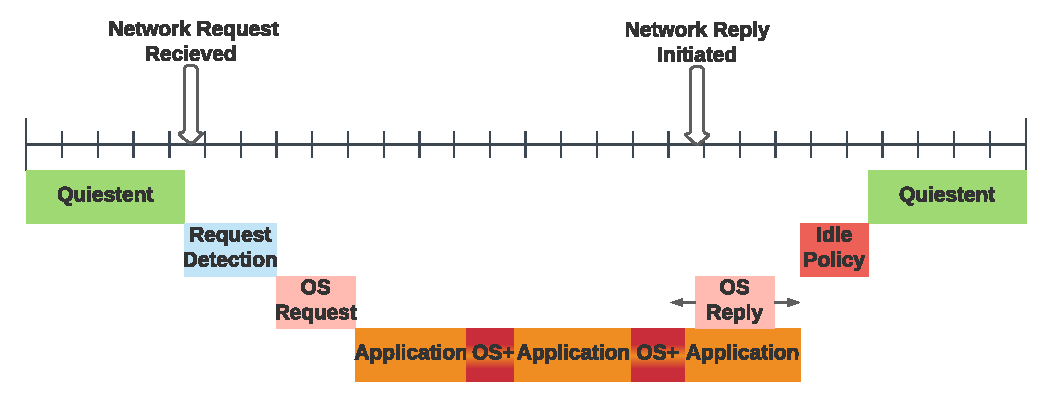
\includegraphics[width=0.5\textwidth]{figures/timeline_chart}
\caption[]{W timeline for a single application request}
\label{fig:timeline}
\end{figure}

From an OS perspective we break down network driven processing into stages that allows us to organize and reflect the OS and application interaction with the workload request timeline.  This break down is illustrated in figure~\ref{fig:timeline}.   

\subsection{Quiescent}
Given the packet and transactional nature of network driven services a quiescent period, in which no requests are present at the server, precedes activity on the server. 

\subsubsection{Open Loop:}
In an open loop scenario like a Memcached workload, the external request rate induces an inter-arrival gap that will drive the quiescent period -- longer at lighter loads (lower queries per second (QPS)) and shorter at heavier loads (higher QPS). Largely the arrival rate can be considered independent of the time required to service a request.  System performance is typically evaluated in terms of the 99\% tail latency it achieves.  Moreover, providers often set a Quality of Service (QoS) target, such as  a 99\% tail latency of 500${\mu}$s, categorizing system performance into acceptable and unacceptable.  As Mootaz et al.\cite{mootaz} observed, in latency focused workloads, the "latency-slack" between the mean time to servicing a request and the QoS target creates an opportunity for energy-performance tradeoffs.  In particular, it maybe possible to reduce mean performance by not executing requests as fast as possible and or not processing request immediately upon their arrival to reduce energy consumption while not violating the QoS target.  

\subsubsection{Closed Loop:}
In a closed loop setting, like snapshotting a database to a remote server or video streaming, the arrival rate of the next request, that forms the overall task, depends on how long it takes to service the current request.  However, the quiescent period is bounded by the network round trip time, that depends on  the size of a request and reply packets, and the remote processing time.   System performance is largely evaluated on how fast a server can complete the entire task given a network link speed and a remote system.  Given workload specific characteristics such as the processing required and round-trip costs it is possible, as we will see, to find configurations in which the OS interacts with slowing down to improve both time and energy.   Often research tends to categorize close loop settings as either not representative of cloud computing or imply that energy-performance tradeoffs are not interesting due to the hight utilization closed-loop processing can imply.  

Given our goal of studying and explaining the implications of the OS on network driven processing our analysis framework, and evaluation, includes closed loop settings.  In particular, we use a simple ping-pong application to stress OS behavior while varying packet-sizes to reveal how OS path length and path efficiency interacts with slowing down processing, relative to the round trip time observed at the server.  Additionally we use a second closed loop that stresses single core application processing with negligible packet sizes to evaluate if OS structure can impact the application efficiency.  

 
\subsection{OS Request Detection}

Fundamental to any operating system is how it detects and schedule processing in response to IO device activity.  At the two extremes are interrupt and poll driven detection.  

\subsubsection{Interrupt driven IO}
Using interrupts has three important implications: 1) Interrupts can be used to transition a processor from a halted state which the OS entered to sleep the processor (at some selected HW sleep state (C-state)) in response to external activity, 2)  Interrupts allow an OS to arbitrate processing across competitive devices and processing in a multi-programmed/multi-device setting, 3) interrupt processing has an inherent performance costs associated with it -- in terms of latency in starting handling of a request, either because of the costs associated with preempting currently scheduled work\cite{intelpaper} or exit penalties associated with the C-state that the processors was halted in\cite{}.  Interrupt processing can also have a negative impact on the instruction efficiency, measured in Instructions Per Cycle (IPC), due to induced micro-architecture hazards such as the inability to prefetch or speculatively execute across an interrupt.

\subsubsection{Poll driven IO}

Most modern high-speed devices expose a memory, if not cache, friendly interface, that permits the processors to read a per-core memory address to determine if the device, such as the Network Interface Card (NIC) has received data that requires processing by the core.  This facility allows software to directly poll the device and initiate software handling without an interrupt.  This approach reduces latency and other performance penalties associated with interrupt driven IO.  However, the period in which the device is checked requires CPU activity and thus limits the ability to halt the cores when there is no work to be done.  In the extreme, a customized OS, supporting a single application can run a poll loop on every core to constantly check for work, conduct the work and then go back to polling for new work and thus never halting the processors due to idleness.   While used in a slightly different context to Kim et al.\cite{hank}, we will refer to this regime as 'no-idle', as it results in a similar energy management strategy albeit in the context of network driven processing.  In general such an aggressive poll approach is assumed to maximize performance by avoiding interrupt overheads and minimizing latency. 

\subsubsection{Hybrid driven IO}
% https://wiki.linuxfoundation.org/networking/napi
A general purpose operating system typically exploits some form of hybrid alternating between using interrupts and polling when servicing high speed NICs. A common strategy is to use interrupts when load is low and switch to polling when load is high and back to interrupts when load reduces.  A general purpose OS, even under sustained high load, bounds the poll phase to avoid the starvation of other devices and computation.  In Linux the framework that implements this hybrid scheme for is called New API (NAPI)\cite{NAPI}.  The first arrival of a packet generates an interrupt which switches the servicing of the device to polling for some budget of packets and time after which the device will no longer be polled and interrupts re-enabled to detect activity on the NIC.  The NAPI framework, in addition to NIC processing budgets,  supports prioritization across devices. 
% In Linux the NAPI polls are processed via softirqs.  Checks for and processing of softirqs happens when ever the system returns to userspace or a hardware interrupt exits.

A library OS that is specialized to support the execution of a single application in the context of a fixed dedicated NICS can explore more extreme strategies like aggressive polling, described above, given that it need not arbitrate the device or cores.

\subsubsection{Interrupt Delaying}
\tikzstyle{startstop} = [rectangle, rounded corners, minimum width=3cm, minimum height=1cm,text centered, draw=black, fill=red!30]
\tikzstyle{io} = [trapezium, trapezium left angle=70, trapezium right angle=110, minimum width=3cm, minimum height=1cm, text centered, draw=black, fill=blue!30]
\tikzstyle{process} = [rectangle, minimum width=3cm, minimum height=1cm, text width=2cm, text centered, draw=black, fill=orange!30]
\tikzstyle{decision} = [diamond, minimum width=3cm, minimum height=1cm, text width=1cm, text centered, draw=black, fill=green!30]
\tikzstyle{arrow} = [thick,->,>=stealth]

%\begin{figure}
\centering
%\resizebox{5cm}{3cm}{%
\begin{tikzpicture}[node distance=2cm]

\node (start) [startstop] {ITR=\textit{n} $\mu$s};
\node (dec1) [decision, below of=start] {ITR==\textit{0}?};
\node (pro1) [process, right of=dec1, xshift=1.5cm] {ITR-=\textit{2} $\mu$s};
\node (dec2) [decision, below of=dec1, yshift=-0.5cm] {RX/TX Event?};
\node (pro2) [startstop, left of=dec2, yshift=1.5cm, xshift=-0.8cm] {Assert Interrupt};

\draw [arrow] (start) -- node[anchor=west] {check} (dec1);
\draw [arrow] (dec1) -- node[anchor=north] {no} (pro1);
\draw [arrow] (pro1) |- node[anchor=west] {update} (start);
\draw [arrow] (dec1) -- node[anchor=west] {yes} (dec2);
\draw [arrow] (dec2) edge[loop right]node{no} (dec2);
\draw [arrow] (dec2) -- node[anchor=east] {yes} (pro2);
%\draw [arrow] (pro2) -| node {} (start);
\draw [arrow] (pro2) |- node[anchor=east] {reset} (start);
\end{tikzpicture}
%}
%\vspace*{-5mm}
%\caption{ITR-Delay algorithm flowchart.}
%\label{fig:itr_delay_flowchart}
%\vspace{-.25in}
%\end{figure}
A common feature of modern high speed NICs is the ability to delay the delivery of interrupt when an event such as packet arrival or transmission completion.  By manipulating this setting software can limit the minimum time between interrupts or in other words the maximum rate at which the NIC events can interrupt the CPUs.    The NIC we use in this study exposes this mechanism via an Interrupt Throttling (ITR) setting.  We flowchart the algorithm from the NIC's datasheet~\cite{82599} in  Figure~\ref{fig:itr_delay_flowchart}. Software uses the ITR register to configure a delay in 2$\mu$s increments.  If the spacing of events, such as packet reception, is less than  $2{\mu}s \times ITR$ the NIC will delay assertion.  If on the other hand events are sufficiently separated an interrupt will be asserted immediately.   

By default the Linux device driver attempts to automatically set ITR to reduce interrupt overheads.  We disable this feature and manually control its value to explore the impact of delaying the detection of NIC events.  Combining interrupt driven IO and delaying interrupt assertion via ITR setting we can explore the impact of delaying packet detection and thus delaying processing of requests.  Depending of the state of the processor the NIC can buffer packets in its own memory or on the main memory of the host\footnote{According to the data sheet if the processor is in sleep state packets can only be buffered on the card's limited memory and once exhausted packets will be dropped}.  Delaying interrupt detection introduces an OS control that can interact with energy and performance.  The prior work of Mootaz et al\cite{mootaz} and the more recently work of Chou et al{chou} suggests that delaying packet processing can interact with DVFS and C-State control in latency sensitive workloads to yield useful energy performance tradeoffs. To this end we sweep ITR values for all our workloads OS configurations, and DVFS values.



%\subsection{Application Perspective}
%Figure~\ref{fig:timeline} shows the application is waiting to be woken up to process new packets (a). Next, an interrupt (b) is fired and the OS network stack begins processing the received packet (c). The application level work begins, alongside there are also interspersed OS work which may or may not be in direct support of application(d). The tail end of the application work (e) typically entails a response packet being sent, the period of time with which the response packet is physically sent can proceed in parallel with the rest of the application level work. The end of every request handling (f) also revolves a set of OS policies to decide the next state of the software and hardware. Work is time spent executing instructions required to service a request, it is a function of the software, hardware, and workload itself. Whereas, idle time is a function of arrival rate of packets.
%
%\subsection{Hardware Perspective}
%Slowing down of the processor causes an increase in the time spent in portions of application and OS work while reducing energy use. Slowing down of interrupt delays contributes to the increase of time spent in the idle states, the longer a processor idles the more energy it can save.
%
%\subsection{OS Perspective}
%OSes overall behaviour is a function of how it behaves during both the working and idle portions of time, there also exists a clear inter-relationship between the two. 
%
%The amount of energy used during this idle period is dependent upon the OS idling policies; in terms of which level of idle state is selected.
%
\subsection{Equations}

%\subsection{ITR-Delay algorithm}


\section{Experiment Setup}
\subsection{Hardware Platform}
Our experimental cluster consists of seven nodes,
each having 16-core processors of either 
Intel(R) Xeon(R) CPU E5-2690 @2.90GHz
or Intel(R) Xeon(R) CPU E5-2650 @2.60GHz type.
All processors have Intel Corporation 82599ES 10-Gigabit SFI/SFP+ NICs,
and all nodes are configured with a mix of 126 GB and 250 GB RAM.
The node we use to boot into our baremetal library OS and Linux server applications uses a Intel(R) Xeon(R) CPU E5-2690 @2.90GHz processor with 126 GB of RAM.

We ensured hardware hosting Linux and the library OS
are setup in a similar way by carefully configure IA-32 Architectural MSRs and processor specific MSRs
(see Tables 35-2 and 35-18 in ~\cite{intel_msr})
as well as NIC features:
direct-cache injection (DCA) disabled,
receive-side scaling (RSS) enabled
(to distribute packets for multi-core processing),
and hardware checksum offloading enabled.
We also match the values of
the number of NIC transmit and receive descriptors
and write-back thresholds for packet transmissions.
Additionally, to minimize system noise, hyperthreads and TurboBoost are disabled on all processors. While prior studies have included TurboBoost in performance-energy studies~\cite{udpm, pacingtoidle, PerAppPower, ixcp}, there have also been reports of energy anomalies when used with different sleep states~\cite{slowdownorsleep}. We use the standard RAPL hardware registers on Intel processors to read per package energy values~\cite{intel_rapl, rapl}.

\subsection{OS Software}
\label{sec:OS}

\subsubsection{Linux}
\label{sec:OS_linux}
%In order to ensure a fair comparison our single-purpose library OS and general-purpose Linux, 
We build a set of application-specific Linux \textit{appliances} for our four workloads. Reminiscent of library OSes~\cite{unikernels}, these appliances are specially constructed to run a RAM-based filesystem and contain only a small set of system libraries and kernel modules required to run their constituent applications. We construct these appliances from a base Debian 10.4 distirbution and use a custom 5.5.17 kernel which we build using a modified configuration file created for supporting high performance, following suggestions from previous work that studies Linux core operation costs~\cite{linux-core-ops}. To avoid scheduling overheads and noise, we pin all applications to physical cores. In addition, we disable Linux ~\textit{irqbalance} and affinitize packet receive interrupts to their respective cores.

\subsubsection{Library OS}
\label{sec:OS_libos}
%% refer back to timeline, this OS structure lets us do this etc.
The library OS used in this work was previously published at OSDI and is currently open-sourced on github (anonymized for now). The library OS consists of specialized components written in C++\footnote{ All components are multi-core functional and optimized to aggressively use per-core memory and fine grain locking.}, including a NIC driver, a custom TCP/IP stack, virtual and physical memory allocators\footnote{Memory allocators make aggressive use of large pages and pinned memory to avoid page-faults.}, and a generic I/O buffer\footnote{I/O buffers are designed to enable zero-copy application data processing.} The library OS is packaged as a library of configurable modules and \textit{gcc-5.3.0}-based tool-chain targeting the base components of the OS. 

Applications are ported to it by configuring the necessary OS components and compiling the application source along with any dependent libraries using this tool-chain. This process generates a single application-specific binary that is source and link-optimized with the OS code. Prior studies have indicated the benefits of both compile-time and link-time optimization on library OS function dispatching~\cite{EbbRT}. We built a bare-metal port of the library OS by writing a network device driver for the Intel 82599 NIC. Our bare-metal port enables application-specific binaries to boot directly on our hardware platform. Once booted, OS and application code is executed under a single supervisor privilege domain. The library OS strictly adopts a run-to-completion, event-driven execution model\footnote{All event handlers are run with interrupts disabled and are expected to return back to the event loop.} and bears similarity to other library OSes designed for high-performance network services~\cite{arrakis, seda, ix, EbbRT}.

%~\cite{ix,seda,arrakis,ebbrt}. 

Given the design and implementation for single-application, non-preemptive processing via an optimized OS and application binary, the library OS components can avoid many checks and streamline execution, ranging from interrupt dispatch to application logic. The NIC device driver totals over 3000 lines of code and interfaces with the library OS multi-core TCP/IP network stack\footnote{The device driver programs the NIC using per-cpu queues and interrupts, maintaining the affinity of TCP connections to their respective cores.}. The library OS provides an interface for statically setting interrupt delay values. We use this interface in our study as we sweep across interrupt delay values. The NIC driver also exposes a configurable constant (set to 64 for all our experiments) that is used to control how many packets can be processed in a single interrupt invocation before returning to the event-loop of the core on which the interrupt was processed. This behaviour, in turn, introduces a simple bounded per-cpu device-level poll.

%The bare-metal library OS uses sleep state algorithm. If no interrupt events or software events exist, the event-loop of the library OS infers that the system is idle and halts the core to enter the deepest sleep state supported by our hardware (C7). In contrast, upon receiving a packet, the device driver management code, protocol processing code, and application code can be dispatched and run to completion on a single event triggered by a NIC interrupt.  %The library OS' idling and device-polling policies are simple compared to Linux policies. %Our study reveals the contrast between these library OS policies and those applied by Linux through presenting a detailed quantification of execution trends and power events. It uncovers surprising impacts of OS functionality on overall system execution and yields insight on OS-level adaptations for energy-performance goals.
\subsubsection{NIC polling in the library OS without sleep}
%% features of the card that lets us poll - read the in-memory 
The simple run-to-completion, and lightweight event-driven execution model of the library OS allows us to also explore the performance-energy trade-offs of slowing down the processor in the context of a polling loop for packet processing. We use standard techniques to auto clear hardware interrupts and enable a tight polling loop. The loop checks a in-memory data structure in which the NIC updates whenever new packet descriptors are to ready be processed. Due to this tight loop, the library OS will never halt the processor and thus will not use any sleep states.

%Intel's 82599 datasheet~\cite{82599} defines two hardware registers that enable automatic clearing and masking of interrupts per receive and transmit queue. To enable polling, we 1) enable auto clearing of network interrupts in order to receive the very first interrupt of every queue, and we 2) disable auto masking to prevent future interrupts on that particular queue. Next, we wrote a custom network interrupt handler for that very first interrupt which effectively calls the packet processing function in a tight loop. D To enable interrupts, we enable both interrupt clearing and masking and set the interrupt handler to be a packet processing function instead.

\begin{table}[t]
\centering
\begin{tabular}{l|c|c|c}
  Name & Scenarios & Nature & CPU\\
  \hline
  NetPIPE & {\small 64B,8KB,64KB,512KB} & CL & Low\\ \hline
  NodeJS & na & CL & High \\ \hline
  Memcached & 200K, 400K, 600K & OL & Low \\ \hline
  Memcached-Silo & 50K, 100K, 200K & OL & High \\ 
\end{tabular}
\caption{Workload configurations.
%NetPIPE and NodeJS are single thread, single connection, closed-loop (CL) workloads. Memcached and Memcached-silo are multiple core, multiple connection, open-loop (OL) workloads.
The column {\em Nature} indicates open-versus-closed loop nature
and {\em CPU} indicates application CPU demand.}
\label{table:wrkcfgs}
\vspace{-.25in}	
\end{table}

\section{Experimental Analysis}
\label{sec:exp}
Figures~\ref{fig:closed_loop_overview}~\ref{fig:mcd_overview},~\ref{fig:mcdsilo_overview} shows an overview of all the experimental datapoints gathered across the different applications and their respective loads as listed in table~\ref{table:wrkcfgs}. For each workload, we break down the differences in slowing down in the respective system types in terms of performance (time for closed-loop and 99\% tail latency for open-loop) and their respective energy use. In order to reason about the trade-offs that occur when slowing down the processor speed and interrupt delay, we use two graphical mechanism to highlight the differences: 
\begin{enumerate}
    \item The \textit{size} of each point is representative of the degree with which the interrupt delay used; the \textit{larger} the size the more interrupt delay is \textit{increased} while the \textit{smaller} the size the more it is \textit{decreased} (faster network interrupts).
    \item The \textit{color gradient} of each point represents the degree of slowing down processor speeds; the \textbf{darker} the color the more the processor has been slowed and vice-versa when the color is \textit{lighter}.
\end{enumerate}

In total, we conducted this study across four system types across the two OSes. For linux and the libOS, the bulk of this work is focused on studying the effects of slowing down processor and interrupts by statically tuning them, and in the figures below, we refer to these datapoints as \textit{LibOS-tuned} and \textit{Linux-tuned}. As a baseline for linux, we tested a configuration where it is not statically tuned (\textit{Linux-default}). For the libOS, we also explored a version of slowing down the processor by replacing network interrupts with a polling loop(\textit{LibOS-poll}). Furthermore, for each of the system type that we've measured, the configuration that yielded the best performance and best (lowest) energy are indicated with a {\larger[4]\textbf{+}} and {\larger[4]\textbf{x}} respectively.

\subsection{LibOS-poll}
The simple run-to-completion, and lightweight event-driven execution model of the libOS allows us to uniquely explore the performance-energy trade-offs of slowing down the processor in the context of a polling loop for packet processing. Intel's 82599 NIC defines two hardware registers that enable automatic clearing and masking of interrupts per receive and transmit queue. To enable polling, we 1) enable auto clearing of network interrupts in order to receive the very first interrupt of every queue, and we 2) disable auto masking to prevent future interrupts on that particular queue. Next, we wrote a custom network interrupt handler for that very first interrupt which effectively calls the packet processing function in a tight loop. To enable interrupts, we enable both interrupt clearing and masking and set the interrupt handler to be the same packet processing function.
\subsection{Closed Loop}
\label{sec:closed_loop}
\begin{figure*}
\centering
%\vspace*{-0.3cm}  
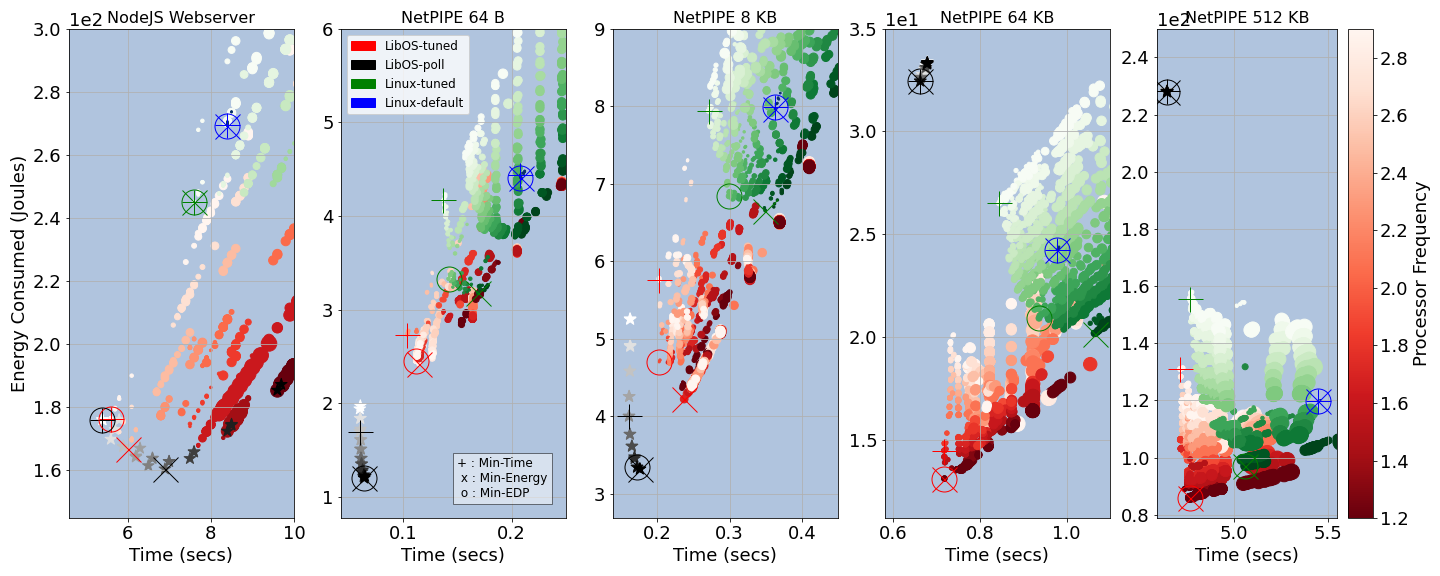
\includegraphics[width=1\textwidth]{figures/closed_loop_overview.png}
\caption[]
%{\small 
{Closed loops.}
\label{fig:closed_loop_overview}
\end{figure*}
\begin{figure*}
\centering
%\vspace*{-0.3cm}  
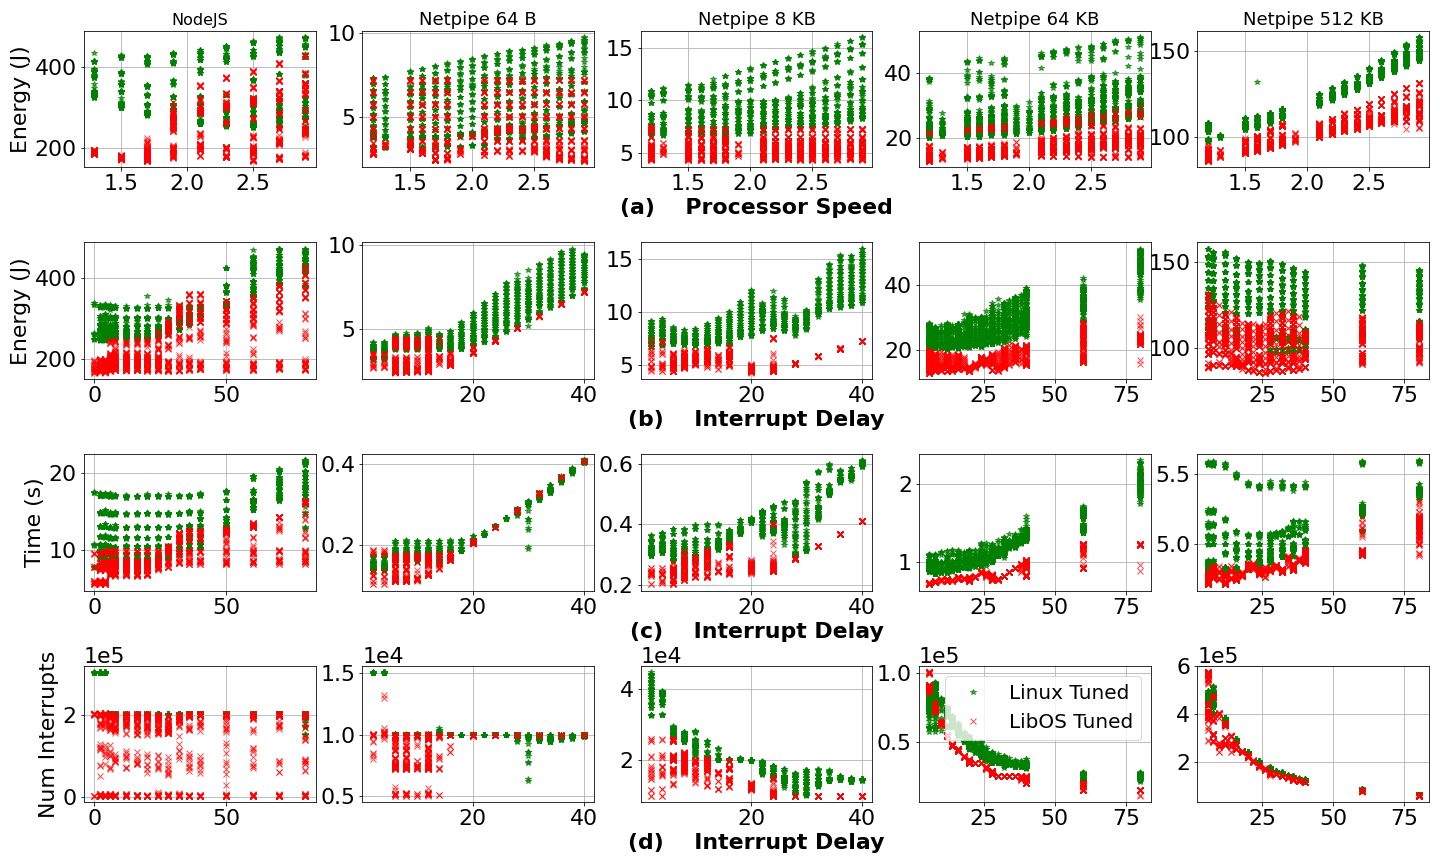
\includegraphics[width=1\textwidth]{figures/closed_detail_1.png}
\caption[]
%{\small 
{Closed loops.}
\label{fig:closed_loop_detail_1}
\end{figure*}
%This approach makes the workloads more predictable and can help smooth out diurnal variations as well~\cite{10.1145/2168836.2168842, 10.1145/2000064.2019527, oldi-study}.
As pointed out in previous studies of energy proportionality in datacenters, the nature of web-centric applications causes diurnal troughs~\cite{Barroso:2009:DCI:1643608, oldi-study, oldi-pegasus, warehouse-power, energyproportion, WebSearch} and one method with which to increase energy efficiency during these troughs is to maximize the amount of work done, typically under a given energy budget. Figure~\ref{fig:closed_loop_overview} illustrates the set of closed-loop workloads studied in our work, all of the workloads are run in a single core with a single connection, further, they enable us to explore these simple closed-loop examples in detail in settings of computationally intensive (nodejs) and across varying network bandwidth requirements (netpipe). Netpipe~\cite{snell1996netpipe} involves sending messages of identical size between two systems for a fixed number of iterations. We fix the iteration count at 5000 and show results for a range of message sizes. \footnote{We found that the 10 GB link is close to saturation when a message of size greater 700 KB is exchanged.}. NodeJS~\cite{nodejs} runs a JavaScript HTTP Webserver and consists of a single client, running the \textit{wrk}~\cite{wrk} benchmark\footnote{We modified \textit{wrk} to place a fixed request load of 100K.}, that sends web requests to a server thread for a fixed period of time. The server responds to each request with a small static payload of size 148 bytes. The library OS was ported to support baremetal NodeJS by providing OS interfaces that link with the V8~\cite{v8} JavaScript engine and libuv~\cite{libuv}. We believe these set of workloads will help to simplify the complexity which to compare and contrast the effects of slowing down in the four types of systems listed above.

\subsection{Observation-1: Speed up interrupt delay to induce polling}

\subsection{Finding-1: Slow-to-stay-busy}

\subsection{Trade-offs in when polling}

\subsection{Memcached}
\label{sec:mcd}

\begin{figure*}
\centering
%\vspace*{-0.3cm}  
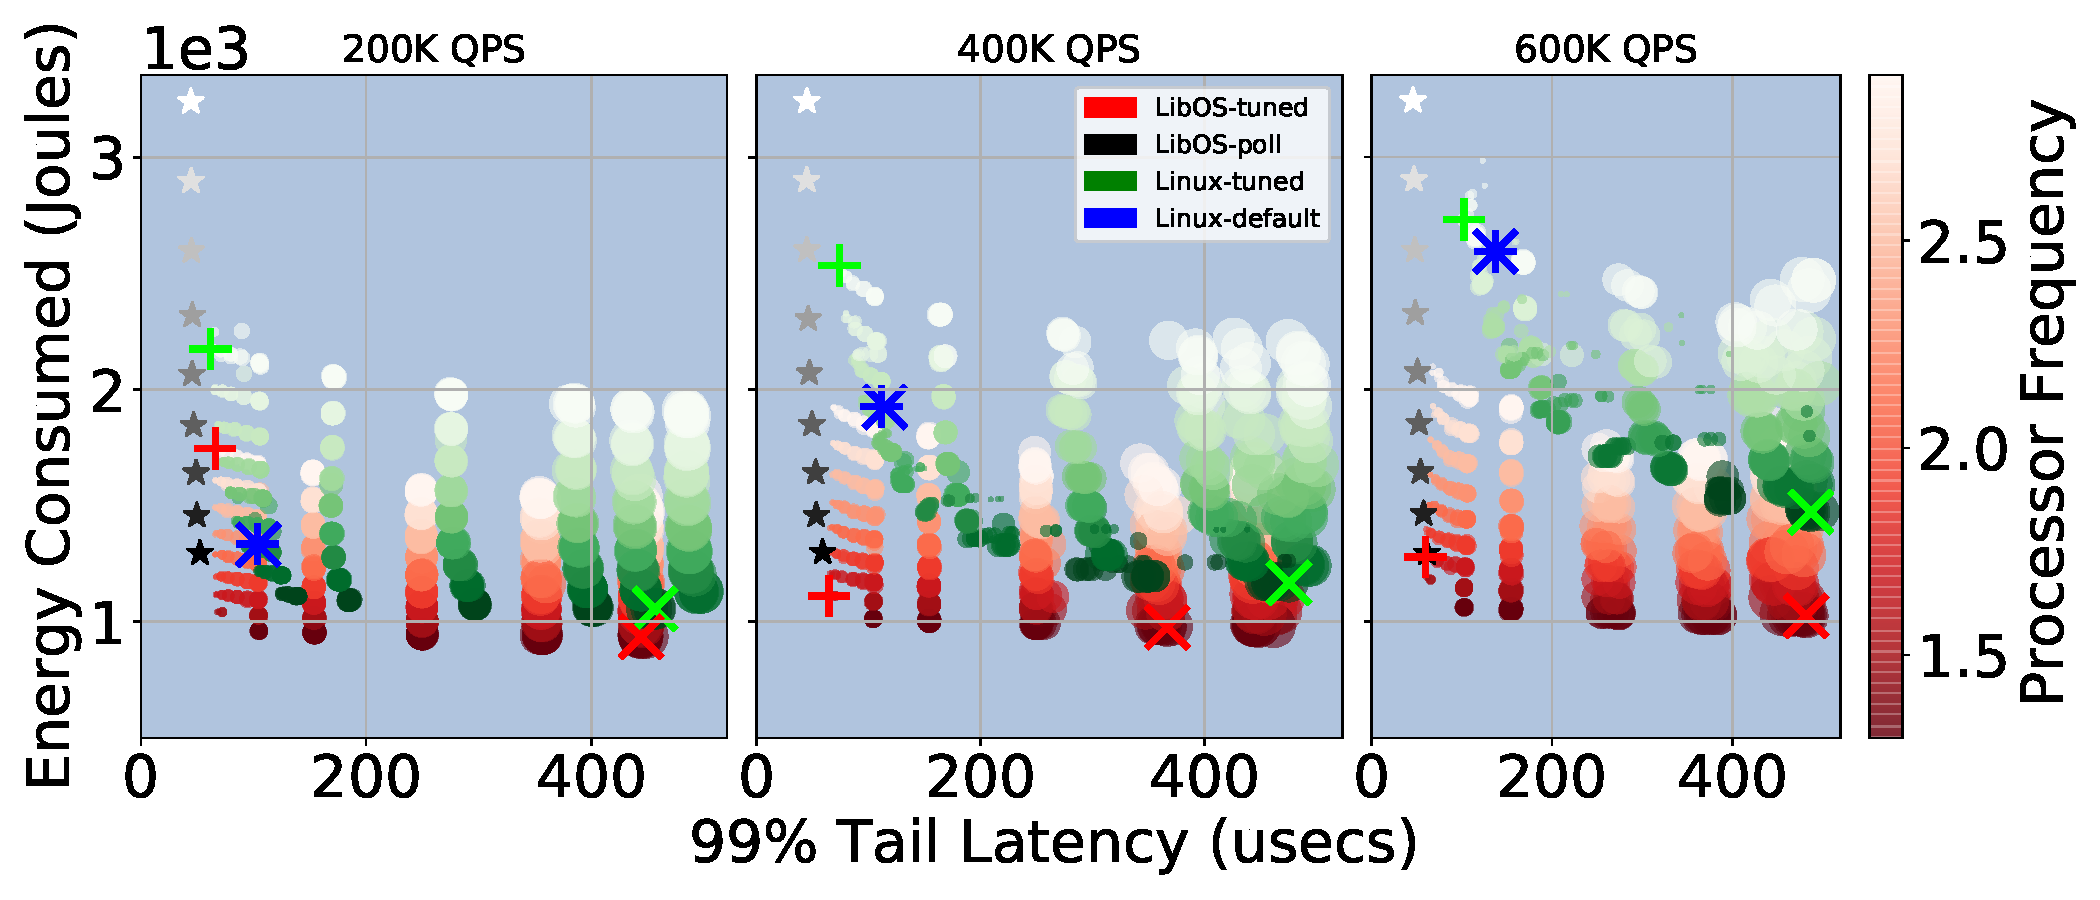
\includegraphics[width=1\textwidth]{figures/mcd_overview}
\vspace*{-8mm}
\caption[]
%{\small 
{Overview of memcached experiments across 200K, 400K, and 600K QPS.
\textbf{x} indicates lowest energy consumption.
\textbf{+} indicates lowest tail latency.}
\label{fig:mcd_overview}
\end{figure*}
\begin{figure}
%\centering
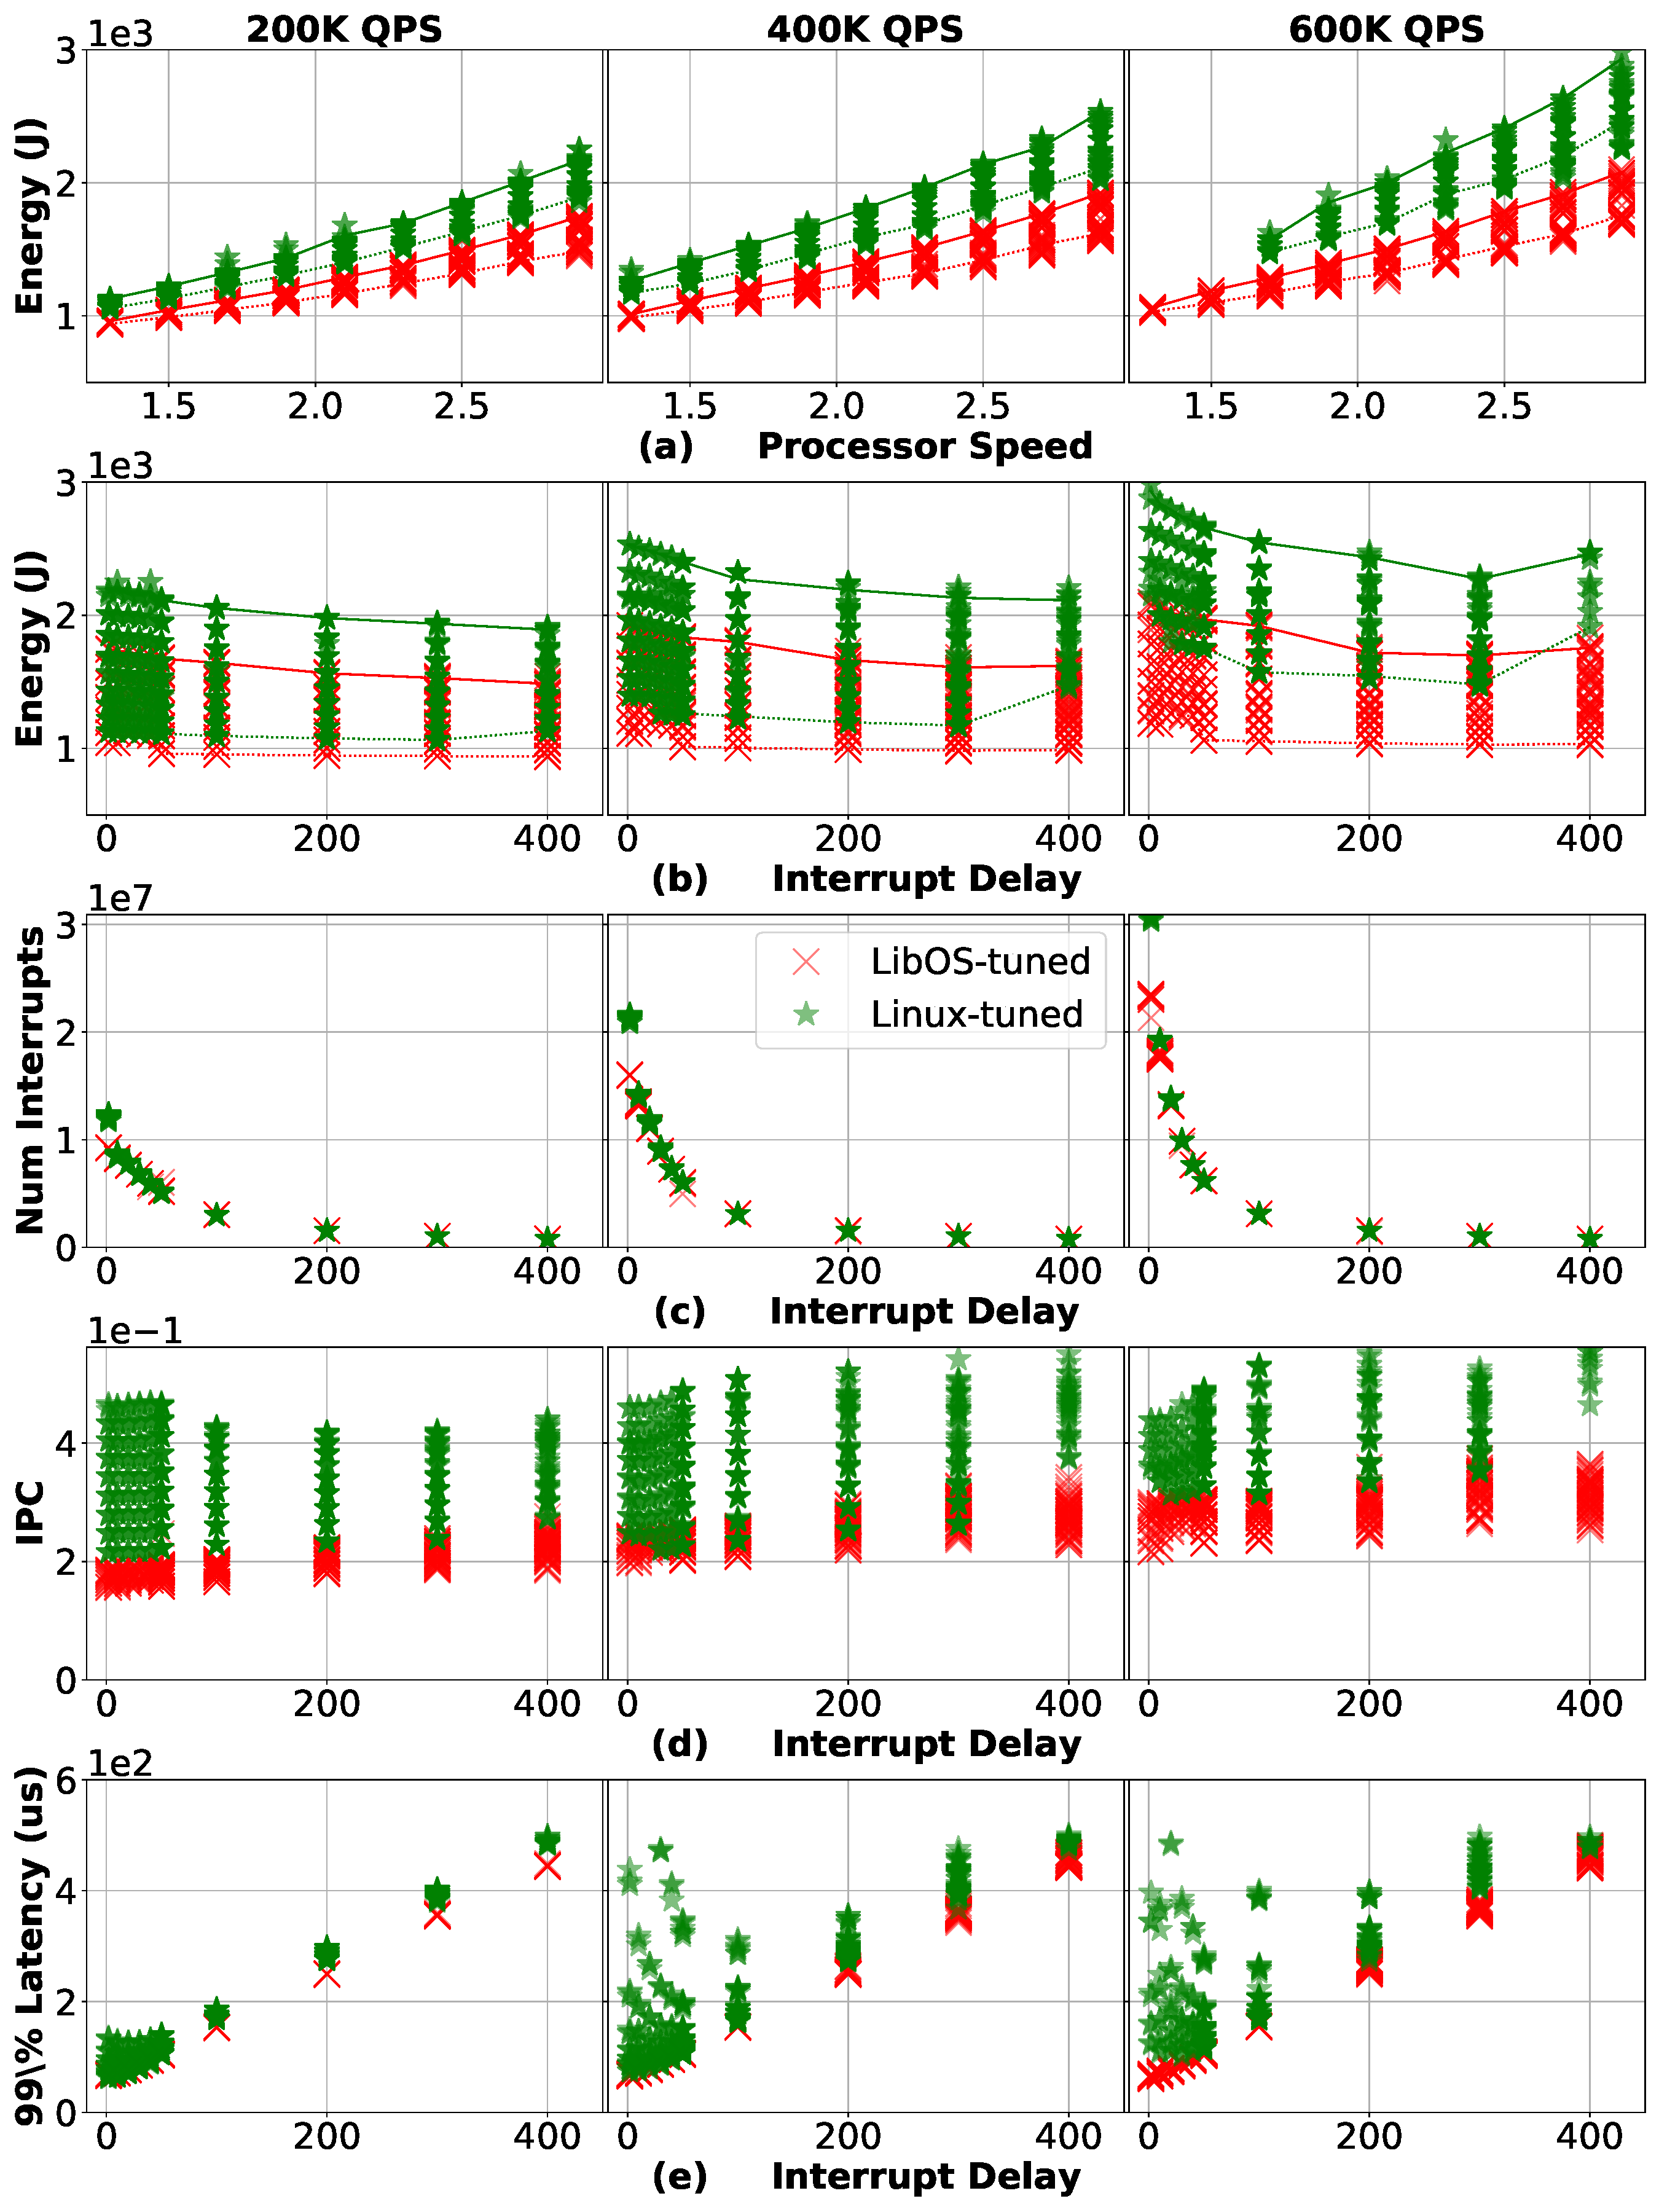
\includegraphics[width=0.5\textwidth]{figures/mcd_detail_1}
\vspace*{-8mm}
\caption[]{Detailed plots of some gathered statistics from experiments with the above QPS loads.
Compares LibOS-tuned and Linux-tuned.}
\label{fig:mcd_detail_1}
\end{figure}
\begin{figure}
%\centering
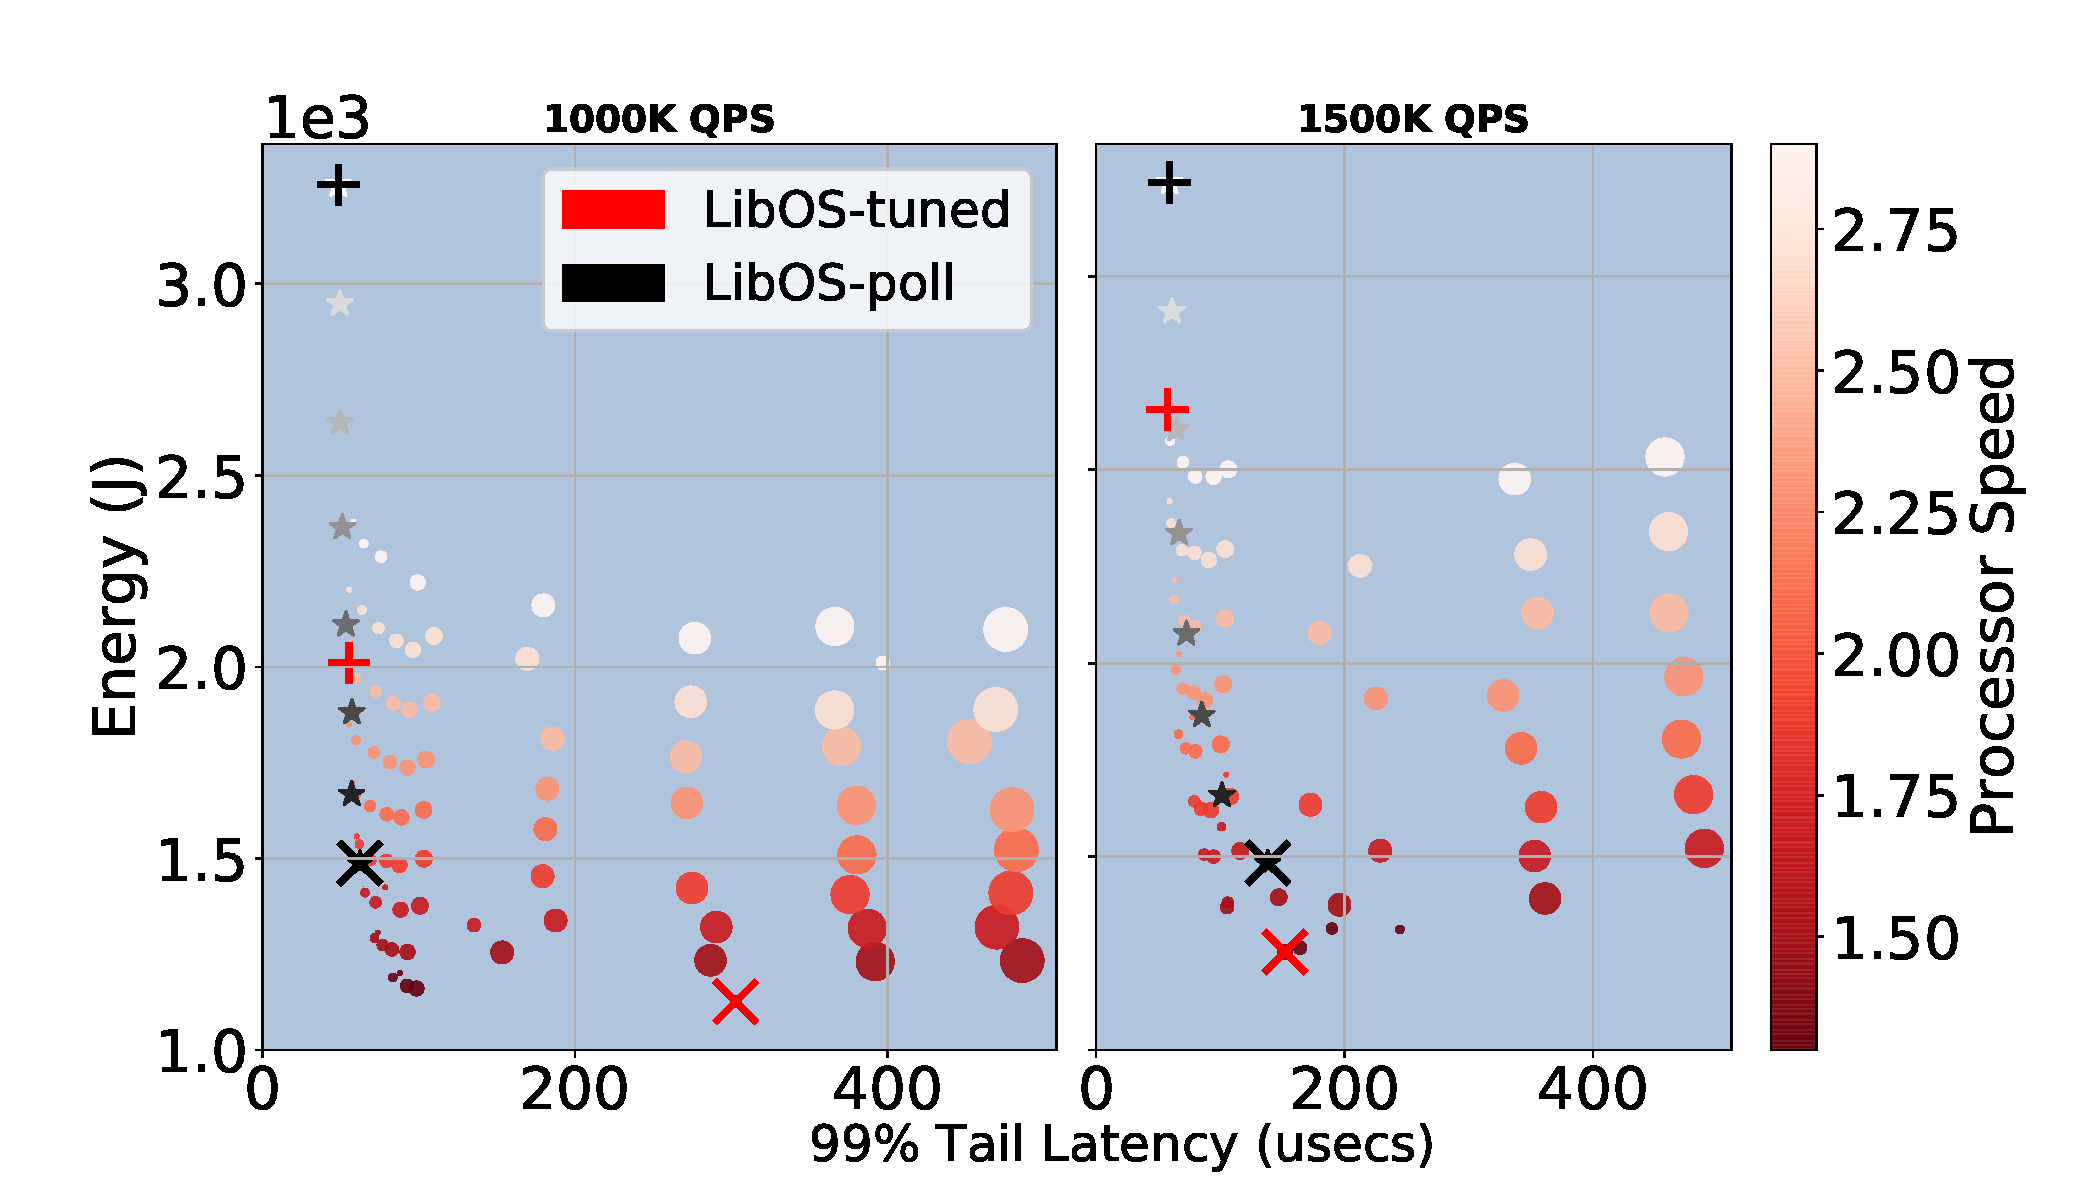
\includegraphics[width=0.5\textwidth]{figures/mcd_overview2}
%\vspace*{-1.0cm} 
\vspace*{-8mm}
\caption[]{Overview of memcached experiments at 1000K and 1500K QPS.}
\label{fig:mcd_overview2}
%\vspace*{-.2in}
\end{figure}
% 200000 ebbrt_tuned 
%  	 SLOW-ITR-diff-Min-Max-DVFS= 702.25 J
%  	 FAST-ITR-diff-Min-Max-DVFS= 544.91 J

% 200000 linux_tuned 
%  	 SLOW-ITR-diff-Min-Max-DVFS= 1041.8 J
%  	 FAST-ITR-diff-Min-Max-DVFS= 760.76 J

% 400000 ebbrt_tuned 
%  	 SLOW-ITR-diff-Min-Max-DVFS= 809.36 J
%  	 FAST-ITR-diff-Min-Max-DVFS= 632.57 J

% 400000 linux_tuned 
%  	 SLOW-ITR-diff-Min-Max-DVFS= 1135.93 J
%  	 FAST-ITR-diff-Min-Max-DVFS= 644.14 J

% 600000 ebbrt_tuned 
%  	 SLOW-ITR-diff-Min-Max-DVFS= 891.97 J
%  	 FAST-ITR-diff-Min-Max-DVFS= 723.47 J

% 600000 linux_tuned 
%  	 SLOW-ITR-diff-Min-Max-DVFS= 706.79 J
%  	 FAST-ITR-diff-Min-Max-DVFS= 547.11 J
Memcached~\cite{mcd} is a multi-threaded open loop workload that runs on all 16 cores of any one of our server nodes. It consists of an unloaded client node running mutilate~\cite{mutilate}. This client (1) coordinates with five other mutilate agent nodes in order to generate requests to the server and (2) measures tail latency of all requests made. All five agent nodes are 16-core machines, whereby each core creates 16 connections, for a total of 1280 connections. This setup is able to saturate the single 16-core server
\footnote{Mutilate is configured to pipeline up to four connections to further increase its request rate.}.

Linux runs memcached-1.6.6 and our library OS uses a re-implemented version of memcached, written to the OS's interfaces, which supports the standard memcached binary protocol. To alleviate lock contention, an RCU hashtable is used to store key-value pairs.
We run a representative load from Facebook~\cite{workloadanalysisfacebook} (ETC) which represents the highest capacity deployment. It uses 20 to 70 byte keys and 1 byte to 1 KB values and contains 75\% GET requests.

%\subsubsection{Slowing down processor has better performance-energy trade-offs for memcached than using sleep states.} 
%\label{sec:mcd:slowproctradeoff} 
%Figure~\ref{fig:mcd_detail_1}(b) shows that even though interrupts are slowed down, the energy differences within each interrupt delay is largely determined by the differences in processor speeds. The bold lines connect the mean energy use of each interrupt delay whereby processor speed is fastest while the dotted lines connect the mean energy use where processor speed is slowest. Compared to figure~\ref{fig:mcd_detail_1}(a), where the differences in energy use is caused by different interrupt delays, we find that reducing energy use by slowing down the \textit{processor} is 2-10X more effective than by slowing down \textit{interrupt delays} (i.e. increased potential for using sleep states) across different QPS rates and OS as well. We believe the main reason is that memcached workloads are bursty with multiple requests pipelined onto multiple cores, therefore the system as whole is always busy with work. This renders potential energy savings by prolonged periods of idleness not as effective as slowing down the processor itself. It should also be noted that Linux at 600K QPS has a smaller energy gap at an interrupt delay of \SI{400}{\micro s} due to the fact that SLA violations already started to occur at faster processor speeds.

\subsubsection{Slowing Down in Different OSes} 
\label{sec:mcd:slowinos}
%Even though figure~\ref{fig:mcd_overview} indicates the libOS uses lower energy than Linux across all QPS loads, we find that in both figures~\ref{fig:mcd_detail_1}(a)(b), Linux is always able to save more energy (1.02X to 3.6X) by slowing down processor and interrupt rates than the libOS. We believe this more a result of the base efficiency of libOS' 
As discussed in section c\ref{sec:workflow:dvfs}, we found that although LibOS-tuned has worse IPC than Linux-tuned across the different QPS loads (figure~\ref{fig:mcd_detail_1}(c)), it also used on average ~2.5X fewer instructions than Linux. Memcached is not a computationally heavy workload; most of its instruction are thus memory bound.
This lowers the effectiveness of slowing down processor in increasing tail latency, given that those instructions are not ALU bound.
The vertical alignment of the library OS points in figure~\ref{fig:mcd_overview} illustrates this ineffectiveness, and we attribute this to the efficiency of the memcached implementation in the library OS system as a whole.

Furthermore, figure~\ref{fig:mcd_overview2} demonstrates that the library OS can support higher QPS loads than Linux due to its specialized OS code paths.
We can see the opposite of this behavior in Linux where, at 600K QPS, Linux approaches 75\% of the peak QPS it can support, and there is a clear trade-off between slowing down processor speeds and an increase in tail latency (higher latency points have darker gradient color).
In figure~\ref{fig:mcd_overview2}, memcached is scaled even higher, to 1500K QPS load, which is around 75\% of the peak QPS that the library OS can support.
At this QPS rate, we can begin to see similar trade-offs in the library OS as in Linux. This finding reveals how a specialized OS's instruction mix can have dramatic implications when slowing down the processor.

% 200000 ebbrt_tuned 
%  	 SLOW-DVFS-diff-Min-Max-ITR= 21.11 J
%  	 FAST-DVFS-diff-Min-Max-ITR= 260.41 J
%  	 FAST/SLOW= 12.3359
% 200000 linux_tuned 
%  	 SLOW-DVFS-diff-Min-Max-ITR= 70.94 J
%  	 FAST-DVFS-diff-Min-Max-ITR= 277.91 J
%  	 FAST/SLOW= 3.9175
% 400000 ebbrt_tuned 
%  	 SLOW-DVFS-diff-Min-Max-ITR= 25.48 J
%  	 FAST-DVFS-diff-Min-Max-ITR= 302.86 J
%  	 FAST/SLOW= 11.8862
% 400000 linux_tuned 
%  	 SLOW-DVFS-diff-Min-Max-ITR= 90.47 J
%  	 FAST-DVFS-diff-Min-Max-ITR= 420.31 J
%  	 FAST/SLOW= 4.6458
% 600000 ebbrt_tuned 
%  	 SLOW-DVFS-diff-Min-Max-ITR= 30.19 J
%  	 FAST-DVFS-diff-Min-Max-ITR= 325.17 J
%  	 FAST/SLOW= 10.7708
% 600000 linux_tuned 
%  	 SLOW-DVFS-diff-Min-Max-ITR= 92.84 J
%  	 FAST-DVFS-diff-Min-Max-ITR= 471.21 J
%  	 FAST/SLOW= 5.0755
\subsubsection{Slowing Down the Processor Diminishes Energy Savings of Sleep States}
\label{sec:mcd:slowprocvssleep}
Figure~\ref{fig:mcd_detail_1}(a) shows that as a processor slows down, the energy savings from slowing down interrupts also decrease.
Bold lines indicate the mean energy use at fastest interrupt delay, while dotted lines indicate mean energy use at the slowest.
We find that across the QPS loads and the two OSes, the average energy savings from slowing down interrupt delay at the \textit{slowest} processor speed is \SI{52}{\joule} while it is \SI{342}{\joule} at the \textit{fastest} processor speed.
 we get a average energy savings of \SI{342}{\joule}.
Detailed in section~\ref{sec:workflow:dvfs}, the effect of slowing down the processor results in the lengthening of the application and OS work in memcached.
This reduces the energy savings that are brought about by taking advantage of sleep states during prolonged idle periods.
Such slow-down is further undesirable due to SLA requirements which result in string time budgets that requests must adhere to.

Even though slowing down interrupt delay does not contribute to energy savings as much as slowing down the processor, figure~\ref{fig:mcd_overview} shows that it is  a combination of both that results in the lowest energy use across both Linux and the library OS.
Figure~\ref{fig:mcd_detail_1}(d) shows the direct effect of interrupt delay on tail latency.
The benefit of slowing down interrupt rates consists of
1) lowering the number of interrupts fired, which also lowers instruction use and potentially promotes better packet coalescing (see figures~\ref{fig:mcd_detail_1}(b)(c)), and
2) ensuring a guaranteed period of quiescence such that the processor can take advantage of potentially deeper sleep states (based off interrupt delay algorithm in figure~\ref{fig:itr_delay_flowchart} and detailed in section~\ref{sec:workflow:itrdelay}).
However, these trade-offs will be different dependent on other factors such as an OS's packet processing efficiency and policies that govern the use of sleep states to maximize quiescence states. Moreover, the benefit of slowing down interrupt rates versus processor speed is a more subtle debate as the implications of slowing down the processor affect all software whereas interrupt delay is a fixed rate that will always wake up the software (if there is work) at some point in the future to handle the interrupt. 

%Manually controlling the interrupt delay value also interacts with sleep state policies in terms of processor wakeup time, sleep state selection, and potential energy-performance trade-offs within this space. 

%Embedded inside the interrupt delay value a
%is an entirely hardware construct outside the purview of software other than knowing at some fixed point in the future to waking up to handle the interrupt.
% Based off these observations, one can assert that to optimize energy savings at a cost to tail latency for memcached involves slowing down both processor and interrupt rate,
%Second, we find that in the libOS, slowing down interrupt rates at the fastest processor speed results in around 11X better energy savings over the slowest processor speed. Similarly we find the same benefits in Linux, however, the energy savings are only around 4X better.


% MIN-TAIL linux_default 200000 1 3.0 135    103.3 1335.43
% MIN-TAIL linux_tuned 200000 2 2.9 135       61.7 2174.6

% MIN-TAIL linux_default 400000 1 3.0 135    111.9 1927.74
% MIN-TAIL linux_tuned 400000 2 2.9 135       74.0 2532.51

% MIN-TAIL linux_default 600000 1 3.0 135    137.5 2594.01
% MIN-TAIL linux_tuned 600000 30 2.9 135     102.6 2730.61

% Linux's network driver contains a interrupt moderation algorithm is a generic algorithm used to cater the interrupt delay rate towards the current traffic pattern to maximize throughput.
\subsubsection{Fast Interrupt Rates Induce Low Tail Latency at High Energy Use.} 
\label{sec:mcd:fastitr} 
Figure~\ref{fig:mcd_overview} also demonstrates the ability to use a low interrupt delay value in order to minimize tail latency. Linux-tuned improved its tail latency over Linux-default by 40\% at 200K QPS and 25\% at 600K QPS. As discussed in section~\ref{sec:workflow:hybridio}, a faster interrupt delay can induce a form of polling with Linux's NAPI policy by constantly waking up the processor to do the OS and application work. This induced behavior also increases energy use by 38\% at 200K QPS and 5\% at 600K QPS which represents another space in the energy-performance trade-off of memcached. While prior research has used static setting of the interrupt delay rate at a low value for experimental stability~\cite{10.1145/2812806, 10.5555/3323234.3323265}, we are the first to show its energy implications.

% MIN-TAIL ebbrt_tuned 200000 2 0x1d00 135        65.9 1747.17
% MIN-ENERGY ebbrt_tuned 200000 400 0xd00 55     444.3  935.44  
% MIN-TAIL ebbrt_tuned 1500000 50 0x1500 135     100.4 1790.14
% MIN-ENERGY ebbrt_tuned 1500000 100 0xf00 135   195.9 1375.67 

% ebbrt_tuned c1 200000 2 0x1d00 135 47.1 1910.13 13115025 9645754
% ebbrt_tuned c1e 200000 2 0x1d00 135 67.4 1772.53 10777190 9203709
% ebbrt_tuned c3 200000 2 0x1d00 135 67.7 1780.14 10747417 9196942
% ebbrt_tuned c7 200000 2 0x1d00 135 68.1 1774.63 10827352 9218834

% ebbrt_tuned c1 200000 400 0xd00 135 442.8 948.19 3291640 781241
% ebbrt_tuned c1e 200000 400 0xd00 135 445.1 941.39 2950100 781239
% ebbrt_tuned c3 200000 400 0xd00 135 445.1 935.63 2676159 781228
% ebbrt_tuned c7 200000 400 0xd00 135 443.8 943.83 3594352 781236

% ebbrt_tuned c1 1500000 0 0x1d00 135 58.5 2633.76 33730121 318342
% ebbrt_tuned c1e 1500000 0 0x1d00 135 59.3 2614.47 31964816 318347
% ebbrt_tuned c3 1500000 0 0x1d00 135 58.9 2640.36 31464117 318348
% ebbrt_tuned c7 1500000 0 0x1d00 135 57.7 2631.38 31876151 318346

% ebbrt_tuned c1 1500000 100 0xf00 135 171.1 1343.02 3939748 312496
% ebbrt_tuned c1e 1500000 100 0xf00 135 191.3 1343.54 3557152 312496
% ebbrt_tuned c3 1500000 100 0xf00 135 196.1 1336.57 3599566 312488
% ebbrt_tuned c7 1500000 100 0xf00 135 195.9 1375.84 3558380 312495
% \begin{table}[t]
% \centering
% \begin{tabular}{l|c|c|c|c|c|}
%   QPS & Type & Sleep State & Latency (\SI{}{\micro s}) & Energy (\SI{}{\joule})\\ \hline
%   200K & Min-Tail & C1 & 47 & 1910\\ \hline
%   200K & Min-Tail & C1E & 57 & 1772\\ \hline
%   200K & Min-Tail & C3 & 67 & 1770\\ \hline
%   200K & Min-Tail & C7 & 68 & 1774\\ \hline
%   200K & Min-Energy & C1 & 442 & 949\\ \hline
%   200K & Min-Energy & C1E & 445 & 941\\ \hline
%   200K & Min-Energy & C3 & 445 & 941\\ \hline
%   200K & Min-Energy & C7 & 443 & 937\\ \hline
%   1500K & Min-Tail & C1 & 58 & 2633\\ \hline
%   1500K & Min-Tail & C1E & 59 & 2614\\ \hline
%   1500K & Min-Tail & C3 & 59 & 2640\\ \hline
%   1500K & Min-Tail & C7 & 58 & 2631\\ \hline
%   1500K & Min-Energy & C1 & 171 & 1343 \\ \hline
%   1500K & Min-Energy & C1E & 191 & 1343\\ \hline
%   1500K & Min-Energy & C3 & 196 & 1336\\ \hline
%   1500K & Min-Energy & C7 & 195 & 1375\\ \hline
% \end{tabular}
% \caption{Min-Tail refers to configuration of processor speed and interrupt rate where the lowest tail latency was achieved and Min-Energy refers to the configuration with lowest energy use.}
% %\caption{Workload configurations.
% %The column {\em Nature} indicates open-versus-closed loop nature
% %and {\em CPU} indicates application CPU demand.}
% \label{table:mcd_sleep_states}	
% \end{table}

% \subsubsection{Finding-5: Sleep states and race-to-halt rarely useful)} \label{sec:f5} 
% Table~\ref{table:mcd_sleep_states} lists a small experiment where different sleep states are explored under the libOS at two extremities when the libOS is lightly loaded (200K QPS) and heavily loaded (1500K QPS). \textit{Min-Tail} is configuring the processor and interrupt rate running fastest while \textit{Min-Energy} is both parameters running slowest. When the libOS is lightly loaded, we find that using different sleep states does make a difference in tail latency and energy. We hypothesize that the small exit latencies of the C1 sleep state results in better tail latencies for memcached. However, we find the effect is lessened when under a heavier load, which seems to indicate that a slowed processor is affecting the efficacy of sleep states given it is already running at a slowed interrupt delay rate, which implies ample opportunities to take advantage of system idling. Moreover, as the load increases for the libOS, selection of different sleep states causes no noticeable differences in either latency nor energy, which implies the constant bursty nature of incoming packets is rendering the idle times non-existent. Lastly, combined with the energy benefits of slowing down the processor versus using sleep states in ~\ref{sec:f2}, we assert that trying to use sleep states for energy savings is largely ineffective. 

\subsubsection{Polling Can be Energy Efficient}
\label{sec:mcd:poll}
Similar to Netpipe with 64B messages (see figure~\ref{fig:closed_loop_overview}), figure~\ref{fig:mcd_overview} shows that using an OS poll for network-bound workloads with a small payload results in the best performance (tail latency) in memcached. Although memcached is a more complex workload than Netpipe with thousands of connections and requests pipelined and multiplexed on multiple cores, LibOS-poll running memcached can still be energy efficient through slowing down the processor. Using \textbf{X} point (Min-Energy) of LibOS-poll as reference, we find that at 200K QPS, LibOS-poll improves both the tail latency and energy over LibOS-tuned at \textbf{+} (Min-Latency) by 20\%. As the load increases, by comparing the Min-Energy points, we find that while LibOS-poll consumes 11\%-38\% more energy across all QPSes, its tail latency was 10\%-90\% better. \textit{Hence a library OS poll reveals an additional trade-off space for energy and performance in memcached}.


% MIN-TAIL ebbrt_tuned   200000 2 0x1d00 135    65.9 1747.17
% MIN-TAIL ebbrt_poll    200000 666 0x1d00 135  44.3 3239.33
% MIN-ENERGY ebbrt_tuned 200000 400 0xd00 55   444.3 935.44 = 415615
% MIN-ENERGY ebbrt_poll  200000 666 0xd00 135   52.4 1296.02 = 67910

% MIN-TAIL ebbrt_tuned   400000 2 0xf00 55      64.9 1111.27
% MIN-TAIL ebbrt_poll    400000 666 0x1b00 135  45.1 2900.71
% MIN-ENERGY ebbrt_tuned 400000 300 0xd00 55   366.6 976.33 
% MIN-ENERGY ebbrt_poll  400000 666 0xd00 135   59.2 1299.53 

% MIN-TAIL ebbrt_tuned   600000 2 0x1100 55     60.2 1278.68
% MIN-TAIL ebbrt_poll    600000 666 0x1d00 135  46.0 3242.68
% MIN-ENERGY ebbrt_tuned 600000 400 0xd00 55   482.0 1025.02 
% MIN-ENERGY ebbrt_poll  600000 666 0xd00 135   61.5 1295.59 

% MIN-TAIL ebbrt_tuned   1000000 2 0x1900 135     55.3 2010.23
% MIN-TAIL ebbrt_poll    1000000 666 0x1d00 135   48.6 3258.35
% MIN-ENERGY ebbrt_tuned 1000000 20 0xd00 135    303.0 1126.13 
% MIN-ENERGY ebbrt_poll  1000000 666 0xf00 135    62.4 1487.28 

% MIN-TAIL ebbrt_tuned   1500000 2 0x1d00 135     57.4 2655.69
% MIN-TAIL ebbrt_poll    1500000 666 0x1d00 135   59.1 3242.74
% MIN-ENERGY ebbrt_tuned 1500000 40 0xd00 135    152.0 1253.26 
% MIN-ENERGY ebbrt_poll  1500000 666 0xf00 135   138.2 1483.45 





%\textbf{Polling - TODO}
%how is it done
%shortened os path length keep it busy during idle periods makes energy lat tradeoff competitive

\subsection{Memcached-silo}
\label{sec:mcdsilo}
Memcached-silo is a open loop workload built on top of the normal memcached protocol. It is computationally and memory more intensive than regular memcached as it incorporates both latency-sensitive network compute and memory-intensive TPC-C style transaction processing. The workload is structured such that on every memcached request, it triggers a corresponding set of TPC-C transaction processing logic on a in-memory database~\cite{silo}. We ported the memcached-silo implementation~\cite{mcdsilo, zygos} to our library OS interfaces. The workload mix and SLA constraints of memcached-silo follow from those used in the memcached experiments in \cref{sec:mcd}. Given its application heavier nature, we only needed two 16-core client nodes at 16 connections per core to saturate a single 16-core memcached-silo server. 

\begin{figure*}
\centering
%\vspace*{-0.3cm}  
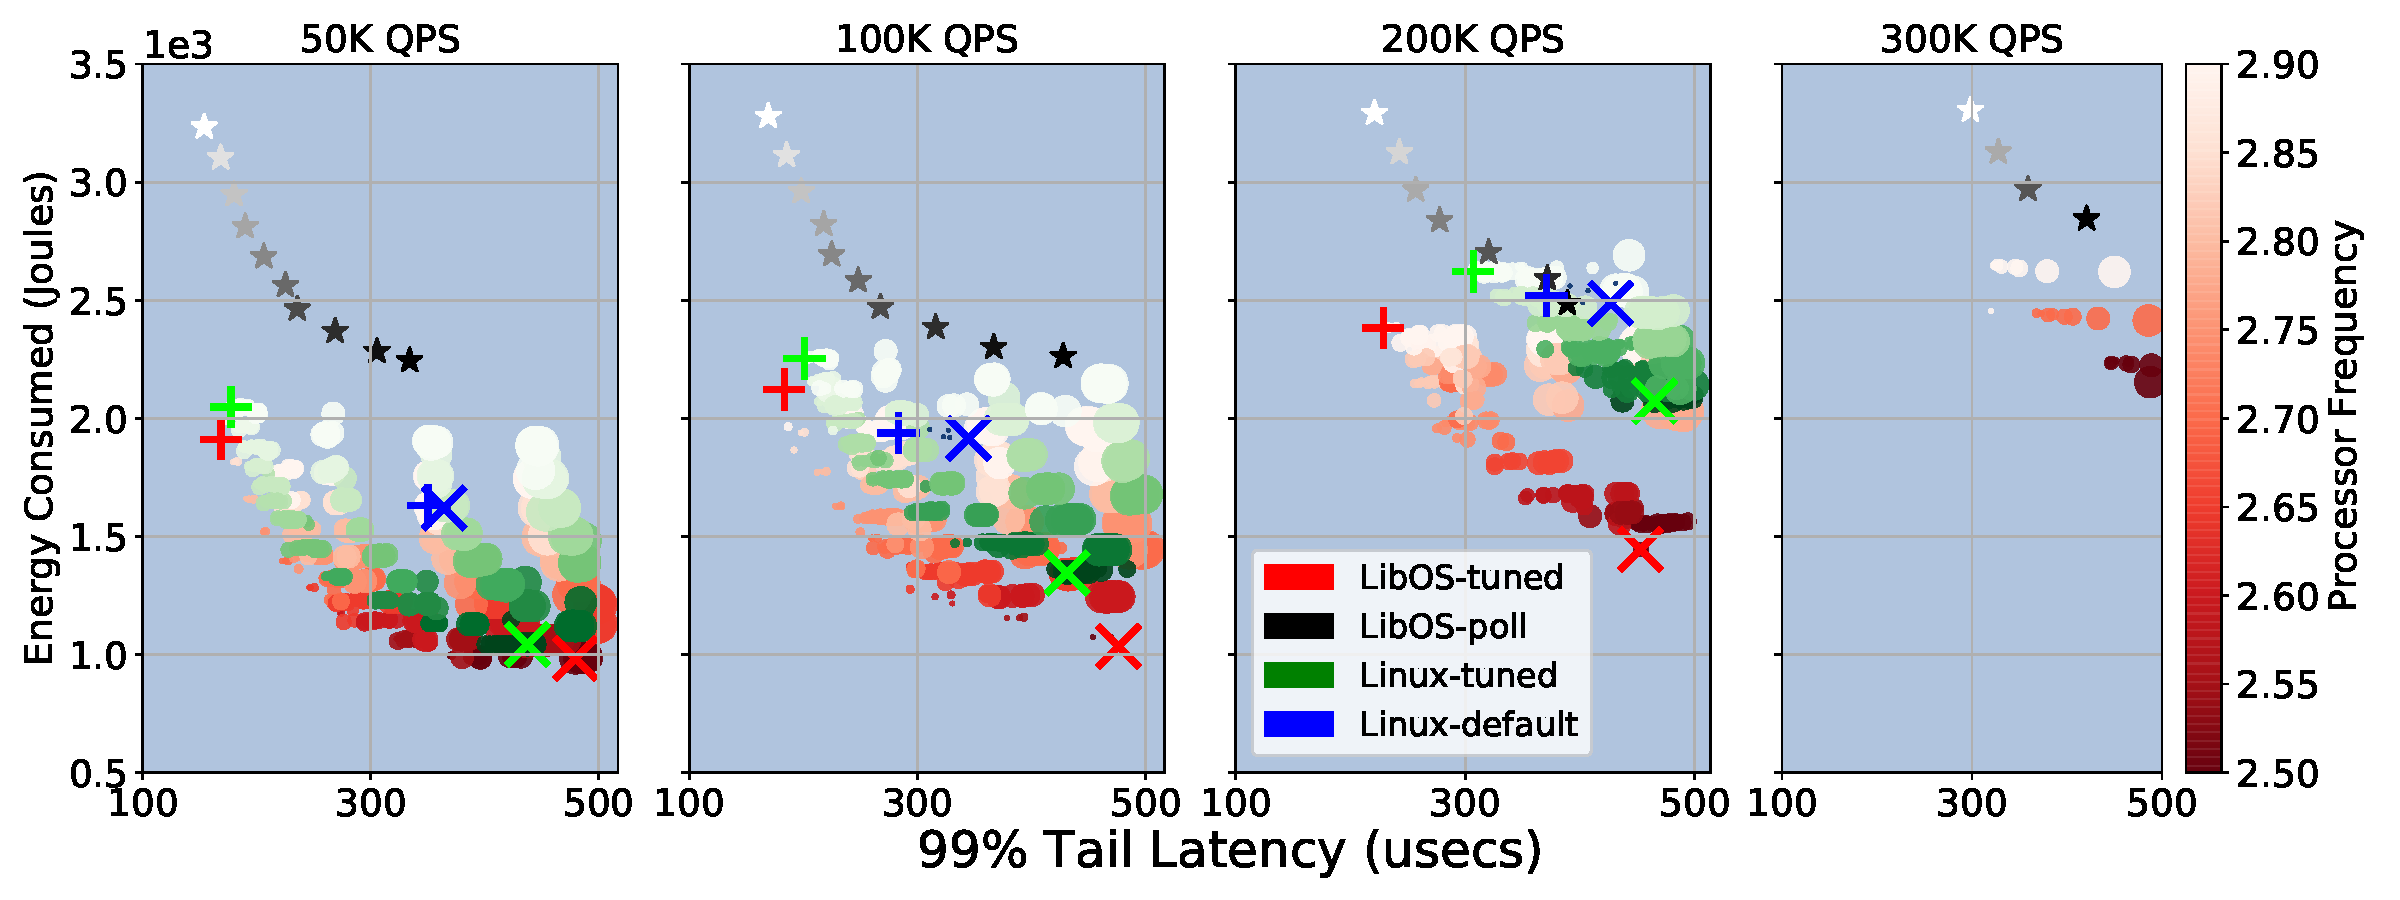
\includegraphics[width=1\textwidth]{figures/mcdsilo_overview}
\caption[]
%{\small 
{Memcached-silo across different QPS.}
\label{fig:mcdsilo_overview}
\end{figure*}

\begin{figure}
%\centering
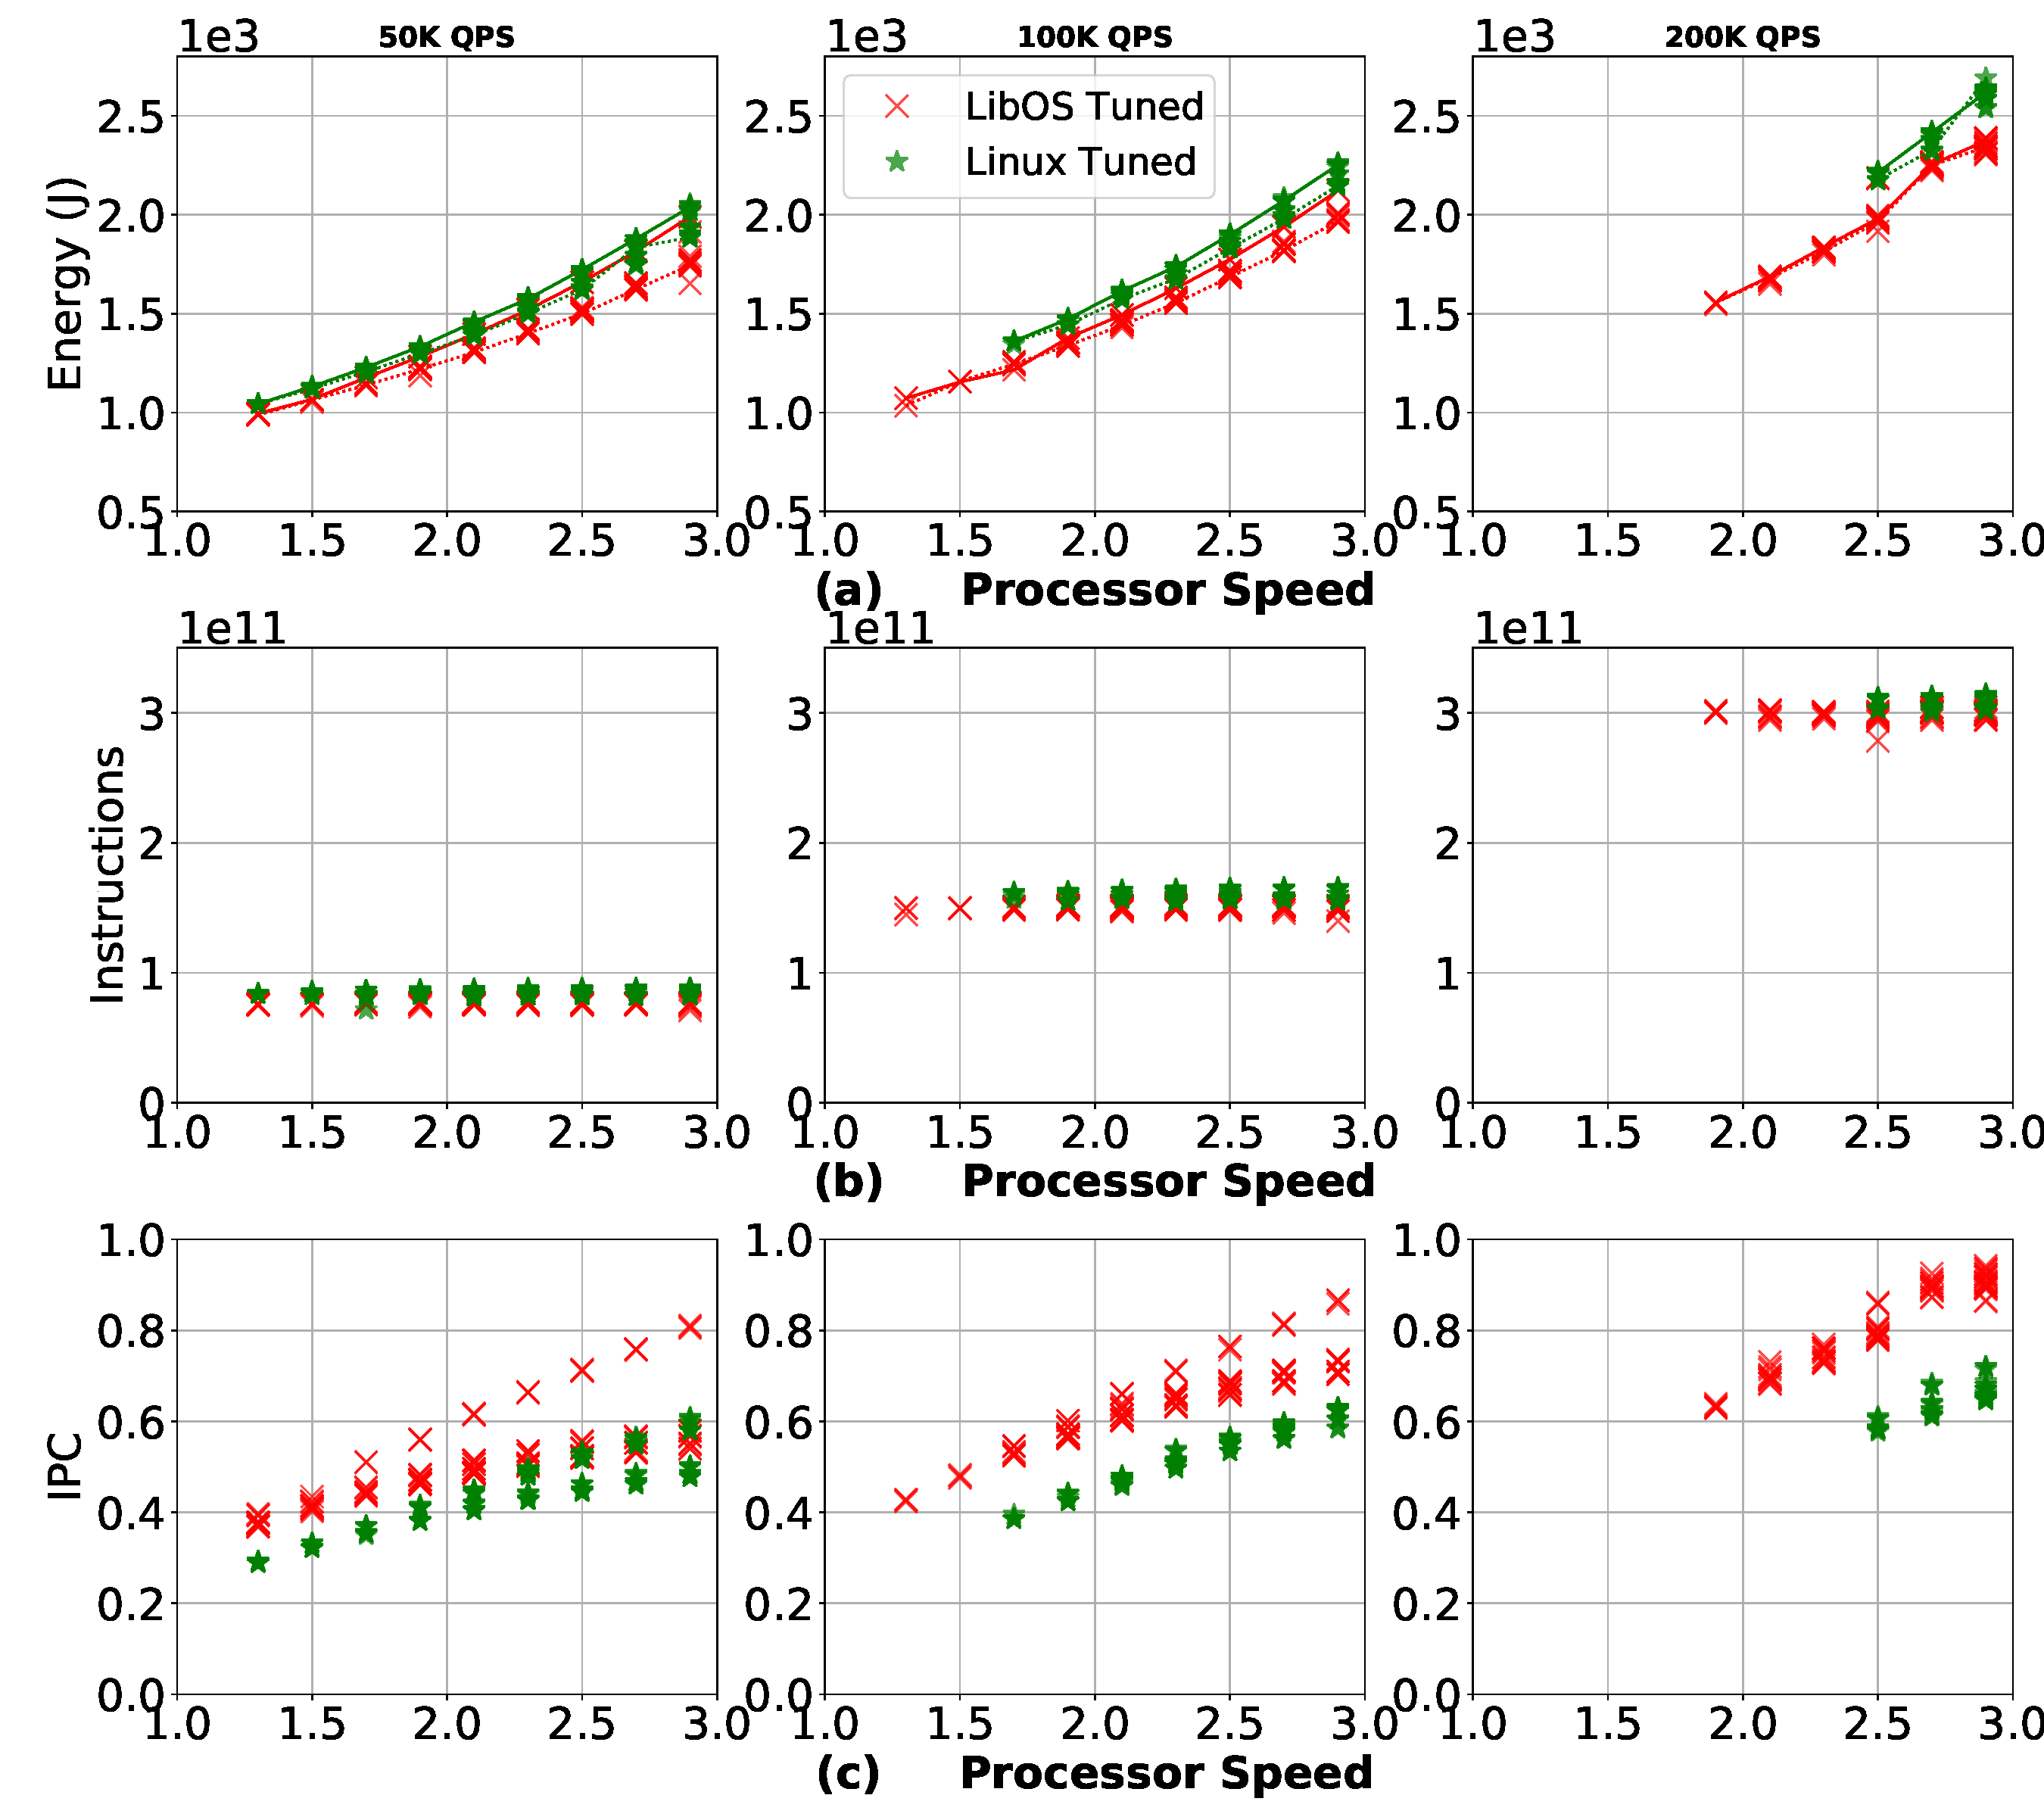
\includegraphics[width=0.5\textwidth]{figures/mcdsilo_detail}
%\hspace*{-10.0cm} 
%\vspace*{-1.0cm}  
\caption[]{}
\label{fig:mcdsilo_detail}
\end{figure}

\subsubsection{similar trade-offs in OSes when application gets heavier}
\label{sec:mcdsilo:dvfstradeoff}

\subsubsection{IPC efficiency, libOS has more headroom}
\label{sec:mcdsilo:ipc}

%\subsubsection{Finding-1: Implications of OS path length efficiency}

% ebbrt_tuned c1 4 0x1d00 135    159.0 1954.58
% ebbrt_tuned c1e 4 0x1d00 135   203.1 1789.93
% ebbrt_tuned c3 4 0x1d00 135    205.2 1779.41
% ebbrt_tuned c7 4 0x1d00 135    206.0 1789.72
% ebbrt_tuned c1 200 0xd00 135   471.5 991.89
% ebbrt_tuned c1e 200 0xd00 135  483.5 990.82
% ebbrt_tuned c3 200 0xd00 135   488.0 987.11
% ebbrt_tuned c7 200 0xd00 135   488.4 989.57

% ebbrt_tuned c1 2 0x1d00 135 304.2 2631.54
% ebbrt_tuned c1e 2 0x1d00 135 312.0 2637.85
% ebbrt_tuned c3 2 0x1d00 135 322.5 2631.96
% ebbrt_tuned c7 2 0x1d00 135 326.9 2646.27

% ebbrt_tuned c1 100 0x1900 135 481.8 2210.25
% ebbrt_tuned c1e 100 0x1900 135 486.1 2051.88
% ebbrt_tuned c3 100 0x1900 135 491.8 2209.09
% ebbrt_tuned c7 100 0x1900 135 492.4 2214.79

% \begin{table}[t]
% \centering
% \begin{tabular}{l|c|c|c|c|c|}
%   QPS & Type & Sleep State & Latency (\SI{}{\micro s}) & Energy (\SI{}{\joule})\\ \hline
%   50K & Min-Tail & C1 & 159 & 1954\\ \hline
%   50K & Min-Tail & C1E & 203 & 1789\\ \hline
%   50K & Min-Tail & C3 & 205 & 1779\\ \hline
%   50K & Min-Tail & C7 & 206 & 1789\\ \hline
%   50K & Min-Energy & C1 & 471 & 991\\ \hline
%   50K & Min-Energy & C1E & 483 & 990\\ \hline
%   50K & Min-Energy & C3 & 488 & 987\\ \hline
%   50K & Min-Energy & C7 & 488 & 989\\ \hline
%   300K & Min-Tail & C1 & 304 & 2631\\ \hline
%   300K & Min-Tail & C1E & 312 & 2637\\ \hline
%   300K & Min-Tail & C3 & 322 & 2631\\ \hline
%   300K & Min-Tail & C7 & 326 & 2646\\ \hline
%   300K & Min-Energy & C1 & 481 & 2210\\ \hline
%   300K & Min-Energy & C1E & 486 & 2207\\ \hline
%   300K & Min-Energy & C3 & 491 & 2209\\ \hline
%   300K & Min-Energy & C7 & 492 & 2214\\ \hline
% \end{tabular}
% \caption{Min-Tail refers to configuration of processor speed and interrupt rate where the lowest tail latency was achieved and Min-Energy refers to the configuration with lowest energy use.}
% %\caption{Workload configurations.
% %The column {\em Nature} indicates open-versus-closed loop nature
% %and {\em CPU} indicates application CPU demand.}
% \label{table:mcdsilo_sleep_states}	
% \end{table}
%\subsubsection{Finding-1: Implications of OS path length efficiency}


\section{Related Work}
\label{sec:related}

% we ask questions regarding OS role in energy proportional computation
The questions that our investigation sparked
fall within a wider space of research
on the impact of OS design
and hardware and software policies
on the incessant goal of energy proportional computation in datacenters
%cite energy proportionality pioneer work:
~\cite{energyproportion, warehouse-power}.
Much of this research stems from
the challenges of improving the performance of
network-bound datacenter workloads
like MapReduce~\cite{large-scale-mapreduce}
and in-memory key-value stores~\cite{mica, zygos}
while keeping energy consumption at bay.
These challenges can be attributed to
the complex diurnal trends
that are characteristic of datacenter-level utilization,
whereby idle time is common and must be optimized for
~\cite{hotpower2008, powernap, napsac}
while simultaneously maintaining the ability to support high-utilization peaks and strict latency constraints
~\cite{Dynamo, SmoothOperator, oldi-pegasus, adrenaline, ixcp, rubik, eurosys14, zygos}.
%smoothoperator
%characterize power fragmentation
%design clstering based approach 



There is a wide range of work
that targets energy proportionality
with a focus on designing OS policies and mechanisms for power management.
Most of this work presents hardware level optimizations
that manipulate active power states (P-states) %cite: p states
and idle power states (C-states) %cite: c states
by applying feedback control mechanisms %cite
and relying on activity models. %cite
%p-states: active power states
Dynamo~\cite{Dynamo}, IX Control Plane~\cite{ixcp}, Pegasus~\cite{oldi-pegasus}, Adrenaline~\cite{adrenaline}, and Rubik~\cite{rubik}
present implementations
that use DVFS %cite
and RAPL %cite
to tune power-draw.
%smoothoperator?
The authors of ~\cite{heracles} and ~\cite{PerAppPower} go a step further,
exploring and characterizing the interference of co-located
latency-critical versus best-effort tasks
and high versus low CPU demand tasks
when subject to energy tuning via DVFS and RAPL.
In doing so,
they highlight limitations
in using hardware features alone for power management.
Similarly, the authors of ~\cite{hotpower2008}
identify a need to step away
from relying entirely on hardware solutions
and focusing instead on software optimizations,
such as VM migration controllers for power management of an ensemble of nodes.
%c-states: idle power states



%notable limitations of p-states and c-states
\cite{oldi-study} presents some of the limitations of
restricting power management to hardware tuning,
and \cite{powercap} compares the merits and limitations of
different hardware and software power management techniques.
These results led us to question
the power management of OS-centric and application-centric tasks
during idle and active utilization
and the majority of time spent in between.
The system is often not idle but only slightly busy,
yet system sleep states present a challenge in
resuming high activity in response to sudden bursts
while system polling maintains support for high activity
but degrades energy efficiency.
%Such challenges motivate research
%on hybrid OS solutions for energy proportional datacenter computation.
In response to this paradox,
the authors of \cite{oldi-pegasus} define an iso-latency policy
that aims to maintain energy proportionality
at variable, dynamically shifting activity levels
via OS-level optimizations.

Though research efforts present significant energy savings
from well designed dynamic policies
and carefully chosen static configurations,
we are driven to explore the space beyond current findings,
with a focus on unveiling the role of the OS
in exploiting activity and idleness.
We find that this exploration is timely
given the range of work on optimizing software components,
from NIC driver mechanisms~\cite{flexnic, affinityaccept, network-latency}
to the OS network stack~\cite{mtcp, sandstorm, network-latency}
and dataplane~\cite{10.1145/299764, 10.1145/2812806},
for energy-efficient large-scale computation.
%INJECT MOTIVATION
Hence we consider an OS-level study
with an interrupt-centric experimental methodology (see \S~\ref{sec:log_collect}) 
for exploring idleness, activity, and the dynamic lapses in between.



%INJECT CONTRIBUTION
This work
started with a motivation to study the impact
of a NIC hardware parameter, ITR-delay,
alongside well studied DVFS and RAPL parameters~\cite{rapl2015, rapl2018},
on energy consumption
of a baremetal libOS in contrast to general purpose Linux.
We wished to quantify the benefits that a libOS,
specialized and optimized for network-bound work,
can have on energy proportionality.
Our efforts concluded with several interesting findings,
one of which is the realization of a potential hybrid solution
for manipulating system idle time in our libOS,
whereby the OS switches from interrupt-driven
%(which assumes clear separation of idle and busy activity)
to polling-driven execution
%(which takes a more intermediary position)
under particular hardware energy configurations.
%add result: less interrupts? more energy saving? better performance?
These findings would not have come to light
were it not for the structure of the libOS
and its particular event-driven execution model~\cite{seda, unikernels}.
%ebbrt
They help us assert that we cannot disregard the OS
as a constituent contributer to application performance and overall cycles-per-instruction (CPI).

%			
%when limitations are reached,
%OS level software optimizations
%--> vm migration
%--> nic controllers
%--> network stacks (libOSes and appliances)
%--> dataplane separation from control plane (ix, arrakis)


%INJECT MOTIVATION
%now the impact of OS path lengths and low level OS behavior becomes primary target for research
%--> hence our motivation for this detailed study of libOS performance vs general purpose linux performance
%--> particularly with emphasis on network and data bound performance

 


\section{Discussion}
\label{sec:dis}
This study involved conducting tens of thousands of experiment runs resulting in approximately four terabytes of data.  Summaries of the data along with all our software is available on github.  Our data includes fine-grain interrupt energy timelines not covered in this paper.  We are in the process of releasing a Python Dash board that allows any researcher to access and navigate our entire data set.  We believe that this paper only scratches the surface of what can be distilled from the data.

% cut if needed
Our study has taught us not only the value of considering energy in OS design and implementation but also demonstrated the ease and value of always gathering energy consumption data.  We encourage all OS research to explore framing all performance results in context of energy as advocated for by mudge~\cite{917539}.

% cut if needed
Our data and it exhaustive sweep based approach reveals several opportunities to construct alternative OS energy management strategies.  For example we now see how valuable it might be to identify when too switch from aggressive polling back to interrupts.  Or how we might switch from using low DVFS settings while on OS paths and then elevate to higher DVFS settings for application code for the application centric workloads.  Additionally it is clear that the phenomena, arising in real settings, of instruction mixes having differing DVFS sensitivities deserves further investigation. 

% cut if needed 
We have presented our mathematical framework in hopes to encourage other researches to continue to build upon it so that both hardware and software researches can identify how changes in behavior can enable better performance while reducing energy.  In appendix~\ref{sec:appendix} we discuss some of th next steps to be take in the development of the framework and usage. 

% cut if needed
Our work also suggests several immediate next steps to enhance our data and mathematical model.  For example it is worth using the library OS to explore a configuration between aggressive polling and interrupts.  In particular using the ability to have the NIC directly awaken a core by writing to a cache-line rather than using an interrupt.   Similarly, the use of different fixed and dynamic sleep states with the library OS.   And finally adding data that documents the behavior of changing DVFS settings at the boundary of OS and application code.  


%\begin{itemize}
%    \item energy data should be elevated and always shown next to performance data, advocated by mudge~\cite{917539}
%    \item all data is on github, we built a dynamic Python Dash web app to look at data
%\end{itemize}
%
%future work:
%\begin{itemize}
%    \item cacheline-based halting
%    \item complex dvfs use when in os and application
%\end{itemize}

% \begin{itemize}
%     \item ITR-delay can be extended up to 1 ms, effect of this on SLAs with 1 ms budget instead?
%     \item As many have observed there is a tension between using controls to throttle processing and thus energy consumption versus the saving that can be had by finishing work quick and halting into lower energy consuming processor sleep states between the requests for work.  The later strategy is often referred to as "race-to-halt" (r2h) while we will refer to the former as "slow-to-stay-busy" (s2sb).  We found that these behaviours, and their effectiveness are largely emergent due to interactions between various interrupt and polling mechanisms and policies.  Additionally, we find that it is possible for a system to effectively modulate between both and that this ability allows the OS to again exploit a wider range of hardware settings over which behaviour can be optimized.
%     \item While it can be very hard to predict how the various hardware setting and software policy modules will interact, there can exist virtuous relationships that can be exploited. A system has many different settings and behaviours that directly on indirectly affect the energy-performance profile.  It is natural in a complex OS for a set of mechanisms and policies to be constructed for a particular category of hardware settings.  Case-in-point being the sleep state that the processor will enter into on execution of the halt instruction.  Our processor defines several such states, each offering a different tradeoff in power consumption and penalties for entry and exit.  Not surprisingly, several mechanism in Linux inter-operate to estimate when to halt and to what sleep state -- including work on the interrupt path used to create an estimate of interrupt arrival and the load induced.  We found, however, that if your OS paths are simple then a fixed halt to deepest sleep state and poll strategy can be sufficient.  The penalty of using the deepest sleep state can be mitigated by modulating the number of halts required by using the processor's throttling controls.   This in turn means that you need not have the complexity added complexity of sleep state management making your system simpler and reducing the number of control points.  But of course to do this you must have the headroom in processing done on every interrupt.   We believe other such opportunities exist ...
% \end{itemize}

% We are the first to quantify the impact of using library OS software on energy.  We find that as expected the library OS uses fewer instruction to complete the work and that this has impact on the energy consumed.  This largely translates into getting more application level work done in fewer instruction and this matters despite the heavy IO nature of the workloads.  This is in part due to the nature of high speed networking.  High speed data center networks put OS device and protocol processing code on the hot path -- in some sense making the workload actually more compute bound that one might expect.  Using fewer instructions (and attendant drop in busy cycles) to complete the application work leads to two energy consumption benefits; 1) it reduces the base energy cost to complete the work, and 2) it creates greater opportunities to halt the processor between network transactions.  The later benefit makes it possible to achieve a simple "race to halt" behaviour across epochs of network activity.  
% Simplistically, by rapidly and efficiently finishing the work required for a network request and sending the reply, one has the opportunity to halt the processor and enter a software specified hardware sleep state\footnote{Processors typically support a range of sleep states where deeper sleep states result in less energy consumption but have higher latency and potential performance penalties when waking up.} till the next interrupt.  The actually, period that one can sleep for depends, as expected, on the workload and the optimization criteria being imposed (eg. latency versus throughput).   

% We also find that across all our workloads, the simplified and naive policies of the library OS, afforded by not needing to run or arbitrate multiple applications, leads to exploiting deeper sleep states while also achieving higher performance.  In EbbRT, when an interrupt occurs, like other library OS it implements a default run to completion model, by disabling interrupts.  When there are no work,  pending interrupts or packets dequeued from prior interrupts to process, EbbRT simply halts the processor to the deepest available sleep state. In contrast, even though we disable Linux's mechanisms for setting the parameters there are other complex algorithms and policies that affect its behaviour.  For example Linux application processing runs with interrupts enabled, it implements a complex algorithm for enacting a hybrid polling versus interrupt processing across network devices and has a subtle infrastructure for deciding what sleep state should be used for halting the processor based on estimation of when the next interrupt will occur from any source.  This all contributes to a complex dynamic behavior with respect to when the system should halt and if it does halt what sleep state will be requested.  We observer that even after we use fixed values for the three  hardware setting considered the other complex behaviours of Linux limits the ability to tune its combined energy and performance compared to EbbRT.


% We identify three hardware settings 

% The components of cloud services such as cache servers, javascript webservers, and in-memory data bases, are  by their nature are network driven.  induce vary degrees of cpu work.  Their operation and thus their efficiency is a complex mixture of the behaviour of the system software and the application software.  While Network Interface Cards (NICs) have many adjustable parameters, Interrupt Delay, the amount of time the NIC will wait before signaling the OS device driver is an value that can easily be changed without any modification to the OS including the device driver.   As expected for a fixed workload this parameter can critically can influence the behaviour of the software for a given workload.  Delaying the packets, depending on the workload the behaviour of the software, one can vary the degree of batching of packets at the expense of increasing the latency of beginning processing a packet. Intuitively, it is possible for a particular workload and software stack their maybe a fixed value that not only optimizes performance but affects the energy consumed as the tradeoff between the frequency of waking up and the amount of work to process on every wakeup can directly influence the efficiency of providing service.  

%  While library Operating systems are one way of catering to a single dedicated application it maybe possible to integrate such support into a general purpose os by adding a new "single app" kernel configuration that disables or sheds run-time complexity and dynamic behaviors to obtain the same benefits we observe.   

\section{Conclusion}
\section{Concluding remarks}

% outline:
%  say briefly what paper did
%  high level results and contributions
%  say unique in fine grained detail 
%  while it is probably obvious, nobody has characterized unikernels
%  conclusions from those resul

We adopt EDP as a metric to improve energy efficiency of network intensive data center workloads. We instrumented code in network device driver to collect packet and hardware statistics at one millisecond granularity. 
We statically tune three hardware parameters DVFS, RAPL and interrupt delay to optimize the EDP for three workloads on both Linux and a library OS. We compared our results to Linux has its dynamic policies enabled. Across the three workloads, we consistently find statically configuring the hardware parameters achieves substantially overall efficiency {\em and} energy efficiency than the dynamic control in default Linux.
%and contrast those statically configured systems to Linux using its normal dynamic heuristics to control those parameters. 

%We find quite consistent results across the four workloads.  First, it turns out that 



%While this is not totally surprising that statically configuring a system that is offering. fixed functionality results in improvements, the degree of improvement is surprising. 
%%In the tuning of Linux we simply turned off its dyanmic control of the hardware mecahnisms, but did not change any of its other dynamic policies.  
%We further found that a special purpose library OS, with no explicit tuning for power, achieve even better energy efficiency.
%To our knowledge we are the first to quantify the impact of using library OS software on energy.

%The study is unique in adopting a very fine grained measurement approach that provides us with insgiht into the behavior of these systems. 
We find that Linux's dynamic policies result in it executing requests rapidly to enable it to quickly go into an efficient deep sleep.
On the other hand, when we statically tune Linux, depending on the demand, it 
can adopt a more efficient mode, finishing the overall work faster and save more energy over Linux default.

%.  That is, it can race to halt on a overall workload rather than in a fine grained fashion.
We are the first to quantify the impact of using baremetal library OS on energy by collecting fine-grained per interrupt statistics of using both packet processing and hardware counters.  We find that the library OS uses fewer instruction to complete the work and that this has impact on the energy consumed.  This largely translates into getting more application level work done in fewer instruction.  High speed data center networks put the OS and protocol stack processing code on the hot path. Using fewer instructions (and attendant drop in busy cycles) to complete the application work leads to two energy consumption benefits; 1) it reduces the base energy cost to complete the work, and 2) it creates greater opportunities to halt the processor between network transactions.  The later benefit makes it possible to achieve a simple "race to halt" behaviour across epochs of network activity and enables going into processor sleep states. We also find that across all our applications, the simplified and naive policies of the library OS leads to taking advantage of faster sleep state transitions while also achieving higher performance. This is due in part to the library OSes packet processing efficiency to get work done quickly and therefore go into a deep sleep state.

%We are the first to explore the impact of a baremetal library OS design on energy efficiency.   We find that as expected the library OS uses fewer instruction to complete the work and that this has impact on the energy consumed.  This largely translates into getting more application level work done in fewer instruction and this matters despite the heavy IO nature of the workloads.  This is in part due to the nature of high speed networking.  High speed data center networks put OS device and protocol processing code on the hot path -- in some sense making the workload actually more compute bound that one might expect.  Using fewer instructions (and attendant drop in busy cycles) to complete the application work leads to two energy consumption benefits; 1) it reduces the base energy cost to complete the work, and 2) it creates greater opportunities to halt the processor between network transactions.  Essentially this enables the library OS to "race to halt" on both an overall workload and per-interrupt basis. 

%Across all our workloads, the simplified and naive policies of the library OS, afforded by not needing to run or arbitrate multiple applications, leads to exploiting deeper sleep states while also achieving higher performance.  In EbbRT, when an interrupt occurs, like other library OS it implements a default run to completion model, by disabling interrupts.  When there are no work,  pending interrupts or packets dequeued from prior interrupts to process, EbbRT simply halts the processor to the deepest available sleep state. In contrast, even though we disable Linux's mechanisms for setting the parameters there are other complex algorithms and policies that affect its behaviour.  For example it implements a complex algorithm for enacting a hybrid polling versus interrupt processing across network devices and has a subtle infrastructure for deciding what sleep state should be used for halting the processor based on estimation of when the next interrupt will occur from any source.  This all contributes to a complex dynamic behavior with respect to when the system should halt and if it does halt what sleep state will be requested.  We observer that even after we use fixed values for the three  hardware setting considered the other complex behaviours of Linux limits the ability to tune its combined energy and performance compared to EbbRT.

This work suggests that, for the fixed function cloud services that dominate today's data centers, externally controlled fixed policies can be much more effective than the complex dynamic policies our operating system's employ today.  It also suggest that there is enormous utility in exploring how we can adopt fixed policies and customized implementations for single applications. While library OSes are one way of catering to a single dedicated application it may be possible to integrate such support into a general purpose OS by adding a new "single app" kernel configuration that disables or sheds run-time complexity and dynamic behaviors to obtain the same benefits we observe.  

The control knobs we tune are external to the OS and result in significant savings. This suggests that statistical learning techniques, especially reinforcement learning methods, would be effective to learn policies geared for specific applications.

%%
%% The next two lines define the bibliography style to be used, and
%% the bibliography file.
\bibliographystyle{ACM-Reference-Format}
\bibliography{references}

\end{document}